\documentclass[12pt,a4paper,oneside]{report}

\usepackage[utf8]{inputenc}
\usepackage[T1]{fontenc}
\usepackage{lmodern}
\usepackage[margin=1in]{geometry}
\usepackage{setspace}
\usepackage{graphicx}
\usepackage{amsmath,amssymb}
\usepackage{booktabs}
\usepackage{longtable}
\usepackage{array}
\usepackage{multirow}
\usepackage{tabularx}
\usepackage{caption}
\usepackage{float}
\usepackage{adjustbox}
\usepackage{microtype}
\usepackage{enumitem}
\usepackage{titlesec}
\usepackage[table]{xcolor}
\usepackage{pifont}
\usepackage[hidelinks]{hyperref}
\usepackage[nameinlink,capitalise]{cleveref}

\onehalfspacing
\setlength{\emergencystretch}{2em}
\graphicspath{{figures/}}
\captionsetup{font=small,labelfont=bf}
\setlist{itemsep=2pt,topsep=4pt}

\titleformat{\chapter}[display]{\normalfont\huge\bfseries}{\chaptertitlename\ \thechapter}{16pt}{\Huge}
\titlespacing*{\chapter}{0pt}{-20pt}{24pt}

\newcommand{\cmark}{\ding{51}}
\newcommand{\xmark}{--}

\begin{document}

% ------------------------------------------------------------------ title
\begin{titlepage}
\centering
{\large\bfseries BACHELOR OF SCIENCE IN COMPUTER SCIENCE AND ENGINEERING\par}
\vspace{3cm}
{\LARGE\bfseries Reliability in Few-Shot Classification with Frozen CNN Adapters: A Controlled Study\par}
\vspace{3cm}
{\large
Hamim Saad Al Raji\\ 210042143\\[6pt]
MD Mainul Hasan\\ 210042173\\[6pt]
Ahmed Sadman Labib\\ 210042135\par}
\vfill
{\large Department of Computer Science and Engineering\\
Islamic University of Technology\\
September, 2026\par}
\end{titlepage}

\pagenumbering{roman}
\setcounter{page}{2}

% ------------------------------------------------------------ declaration
\chapter*{Declaration of Candidate}
\addcontentsline{toc}{chapter}{Declaration of Candidate}
This is to certify that the work presented in this thesis is the outcome of the analysis and
experiments carried out by Hamim Saad Al Raji, MD Mainul Hasan, and Ahmed Sadman Labib under the
supervision of Shahriar Ivan, Assistant Professor, Department of Computer Science and Engineering,
and the co-supervision of Md.\ Bakhtiar Hasan, Assistant Professor, Department of Computer Science
and Engineering, Islamic University of Technology, Dhaka, Bangladesh. Neither this thesis nor any
part of it has been submitted anywhere else for any degree or diploma. Information derived from the
published and unpublished work of others has been acknowledged in the text, and a list of references
is given.

\vspace{1.5cm}
\noindent
{\small
\begin{minipage}[t]{0.58\textwidth}
\rule{6cm}{0.4pt}\\
Shahriar Ivan\\
Assistant Professor\\
Department of Computer Science and Engineering\\
Islamic University of Technology (IUT)\\
Date: September 17, 2026\\[1.4cm]
\rule{6cm}{0.4pt}\\
Md.\ Bakhtiar Hasan\\
Assistant Professor\\
Department of Computer Science and Engineering\\
Islamic University of Technology (IUT)\\
Date: September 17, 2026
\end{minipage}%
\hfill
\begin{minipage}[t]{0.38\textwidth}
\rule{5cm}{0.4pt}\\
Hamim Saad Al Raji\\
Student ID: 210042143\\
Date: September 17, 2026\\[1.2cm]
\rule{5cm}{0.4pt}\\
MD Mainul Hasan\\
Student ID: 210042173\\
Date: September 17, 2026\\[1.2cm]
\rule{5cm}{0.4pt}\\
Ahmed Sadman Labib\\
Student ID: 210042135\\
Date: September 17, 2026
\end{minipage}}

% ------------------------------------------------------------- dedication
\clearpage
\vspace*{\fill}
\begin{center}
\itshape Dedicated to everyone who insisted that a model's confidence should mean something.
\end{center}
\vspace*{\fill}

% -------------------------------------------------------- acknowledgement
\chapter*{Acknowledgement}
\addcontentsline{toc}{chapter}{Acknowledgement}
We are grateful to our supervisor, Shahriar Ivan, Assistant Professor, Department of Computer
Science and Engineering, for his guidance and his patience while this project grew from a single
proof-of-concept episode into a full experimental study. He let our negative results stand as
negative results, and this thesis is better for it.

We are equally grateful to our co-supervisor, Md.\ Bakhtiar Hasan, Assistant Professor, Department of
Computer Science and Engineering, for his advice on the evidential and calibration parts of the work,
and for pushing us toward a cleaner experimental design whenever a shortcut looked tempting.

We thank the Department of Computer Science and Engineering, Islamic University of Technology, for the
environment and coursework that made this research possible. Almost all of our training runs were
done on the free Tesla T4 GPUs offered by Google Colab and Kaggle, and we relied throughout on PyTorch
and the wider open-source Python ecosystem.

Finally, we thank our families and friends for their patience during the months when a screen full of
calibration numbers seemed to us like the most interesting thing in the world.

% --------------------------------------------------------------- abstract
\chapter*{Abstract}
\addcontentsline{toc}{chapter}{Abstract}
Parameter-efficient fine-tuning (PEFT) adapts a pretrained network by training only a small add-on
module, and it is usually judged by accuracy alone. In few-shot image classification on small devices,
accuracy is not enough: the model's confidence should be trustworthy and it should notice inputs that
belong to none of the known classes. This thesis is a controlled study of which design choices govern
which of these properties when a frozen, ImageNet-pretrained lightweight CNN (ResNet-18 or
MobileNetV3-Small) is adapted with a small trainable adapter (a parallel bottleneck or LoRA, at most
31.7K parameters) and classified by a parameter-free prototype head whose logits are read either as a
softmax or as evidential (Dirichlet) evidence. We train a balanced factorial grid of 120 models (five
two-level factors, two baselines, three seeds) on 5-way 1- and 5-shot CIFAR-FS and MiniImageNet
episodes and measure accuracy, calibration (ECE) and out-of-distribution detection (AUROC against four
OOD sets per dataset). Four questions are asked of this grid. First, shot count explains about 76\% of the
variation in accuracy and head type about 83\% of the variation in calibration, while the head barely
affects accuracy. Second, when every model is scored with every uncertainty score, the scoring rule
explains 42.7\% of far-OOD variation and the training objective only 0.17\%; the parameter-free energy
score is the strongest score in most settings. Third, a pre-registered experiment that gives both
adapters the same parameter budget shows that accuracy follows adapter architecture (the bottleneck
wins 8 of 8 comparisons) whereas the calibration gap follows the backbone, not the budget (budget
hypothesis supported in 0 of 4 cells, backbone dependence in 3 of 4). Fourth, refitting only the two
evidence parameters of the evidential head on validation episodes improves its calibration in all 60
models (mean ECE 0.323 to 0.185) but does not bring it level with softmax, and does not lower OOD
AUROC by more than 0.005 in 80\% of comparisons. No single design choice makes the model reliable on every
axis; what the thesis offers is a map of which choice controls which property.

% ------------------------------------------------------------------ lists
\tableofcontents
\listoffigures
\listoftables

\chapter*{List of Abbreviations}
\addcontentsline{toc}{chapter}{List of Abbreviations}
\begin{tabular}{@{}ll@{}}
AUROC & Area Under the Receiver Operating Characteristic Curve\\
CNN   & Convolutional Neural Network\\
ECE   & Expected Calibration Error\\
EDL   & Evidential Deep Learning\\
FPR@95 & False Positive Rate at 95\% True Positive Rate\\
FT    & Fine-Tuning\\
ID    & In-Distribution\\
KL    & Kullback--Leibler (divergence)\\
LoRA  & Low-Rank Adaptation\\
MSP   & Maximum Softmax Probability\\
NLL   & Negative Log-Likelihood\\
OOD   & Out-of-Distribution\\
PEFT  & Parameter-Efficient Fine-Tuning\\
TIN   & TinyImageNet\\
TS    & Temperature Scaling\\
ViT   & Vision Transformer\\
\end{tabular}

\clearpage
\pagenumbering{arabic}

\chapter{Introduction}
\label{ch:intro}

Small devices increasingly have to recognise categories they were never trained on, often from one
to five labelled photos per new category. A practical way to do this is to take a network pretrained on
a large dataset, freeze it, and train only a small add-on module, an \emph{adapter}. Such adapters are
usually evaluated by one number, accuracy. This thesis asks what happens to the other parts of
reliability, namely whether the model's confidence can be trusted and whether it notices inputs that do
not belong to any known class, and which design choices control each of them.

\Cref{tab:headline} previews the answer. Each reliability aspect turned out to be controlled by a
different design choice, so no single choice makes the model reliable on every axis.

\begin{table}[H]
\centering
\caption{Which design choice governs which reliability aspect (details in \cref{ch:results}).}
\label{tab:headline}
\begin{adjustbox}{max width=\textwidth}
\begin{tabular}{@{}ll@{}}
\toprule
Reliability aspect & Governed mainly by \\
\midrule
Accuracy & shot count, then adapter architecture \\
Calibration & head type, then backbone \\
OOD detection & the uncertainty scoring rule \\
Repairing evidential calibration & a two-parameter post-hoc refit helps, but does not fully fix it \\
\bottomrule
\end{tabular}
\end{adjustbox}
\end{table}

\section{Background and Motivation}

Convolutional networks pretrained on ImageNet~\cite{deng2009imagenet} learn features that transfer
well to new visual tasks. The usual way to reuse them is full fine-tuning, which updates every weight.
When the new task has only a handful of labelled images per class, this is risky: a model with millions
of free parameters can fit five images in many ways, most of which do not generalise. This is the
setting of few-shot learning, where a model sees $K$ labelled examples per class (usually $K \in
\{1,5\}$) and must then classify new images of those classes~\cite{vinyals2016matching}.

Parameter-efficient fine-tuning (PEFT) keeps the pretrained network frozen and trains a small number of
new parameters instead. Bottleneck adapters~\cite{houlsby2019adapters} and low-rank adaptation
(LoRA)~\cite{hu2022lora} can approach the accuracy of full fine-tuning while training a tiny fraction of
the weights. Most of this work, however, targets large transformers on data-rich benchmarks. Lightweight
CNNs remain the practical choice for many edge devices~\cite{somvanshi2025tinydl}, and how adapters
behave inside them under few-shot scarcity has received much less attention.

Accuracy is also only one part of reliability. A model that says it is 95\% sure while being right
60\% of the time is \emph{miscalibrated}, and modern networks are known to be overconfident in this
way~\cite{guo2017calibration}. A related requirement is \emph{out-of-distribution (OOD) detection}:
recognising that an input belongs to none of the known classes instead of confidently assigning it to
one of them~\cite{hendrycks2017baseline}. Evidential deep learning (EDL)~\cite{sensoy2018edl} offers one
way to express this kind of uncertainty: the network outputs evidence for each class, which defines a
Dirichlet distribution, and a low total amount of evidence signals ``I don't know'' in a single forward
pass.

This thesis brings these threads together. We adapt frozen lightweight CNNs with small adapters, read
the output either as a softmax or as evidential evidence, and measure accuracy, calibration and OOD
detection on the same trained models.

\section{Problem Statement}

The study starts from one observation: a model can be accurate and still unreliable.
\Cref{fig:reliability} shows the two failure modes we measure. On the left, a known-class input is
misclassified with high confidence; on the right, an input from an unseen class is confidently assigned
to a known class. Neither failure shows up in an accuracy number.

\begin{figure}[H]
\centering
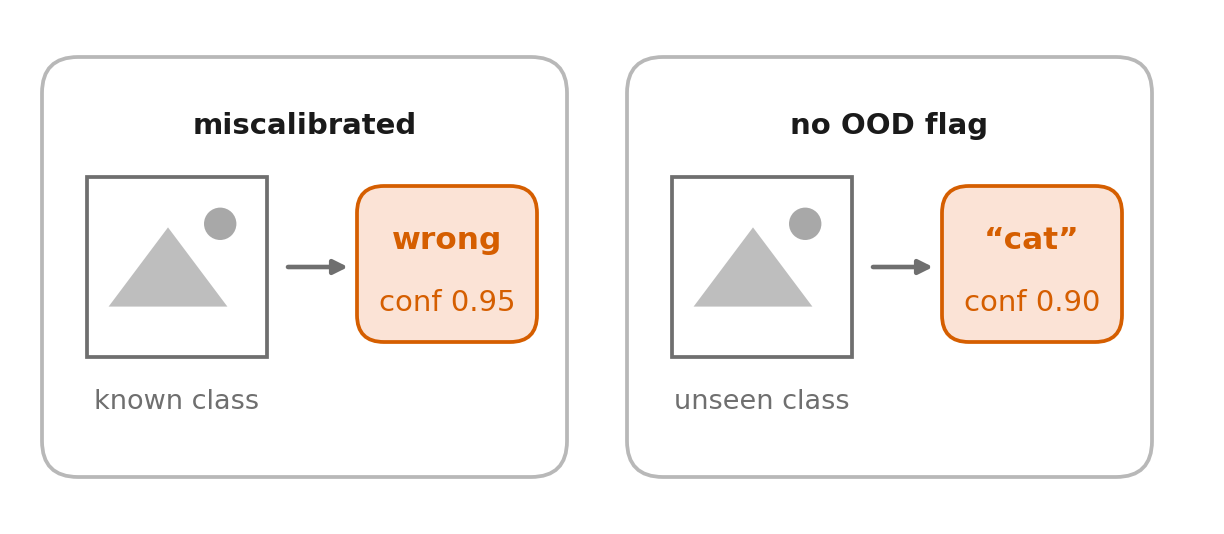
\includegraphics[width=0.85\textwidth]{D1_accuracy_vs_reliability.png}
\caption{Accuracy is not reliability. Left: a known-class input confidently misclassified
(miscalibration). Right: an input from an unseen class confidently assigned to a known class (no OOD
flag).}
\label{fig:reliability}
\end{figure}

Three gaps motivate the work:
\begin{itemize}
\item \textbf{Full fine-tuning is expensive and fragile in the few-shot regime.} It updates millions of
weights from a few images per class and must be stored per task.
\item \textbf{PEFT studies rarely measure reliability.} Adapter papers usually report accuracy only, so
it is unclear what an adapter does to confidence and OOD behaviour.
\item \textbf{PEFT research focuses on transformers.} Adapters, LoRA and prompt tuning were developed
for and mostly evaluated on transformers~\cite{houlsby2019adapters,hu2022lora,jia2022vpt,chen2022adaptformer}.
CNN-side work exists~\cite{chen2024convadapter,li2022tsa,aleem2024convlora,zhong2024convlora} but rarely
combines PEFT with calibration and OOD evaluation.
\end{itemize}

\Cref{tab:challenges} pairs each gap with the design decision we take in response. This is an
evaluation study, not a new model: we use existing adapters and heads and compare them under one
controlled protocol.

\begin{table}[H]
\centering
\caption{The three gaps and how this thesis responds to each.}
\label{tab:challenges}
\begin{tabularx}{\textwidth}{@{}>{\raggedright\arraybackslash}p{5.2cm}X@{}}
\toprule
Gap & Our response \\
\midrule
Full fine-tuning updates millions of weights & Freeze the backbone and train at most 31.7K adapter
parameters once. New classes need no further gradient steps. \\
PEFT studies rarely measure reliability & Measure accuracy, calibration and OOD detection on the same
runs. \\
PEFT research focuses on transformers & Study adapters inside frozen lightweight CNNs. \\
\bottomrule
\end{tabularx}
\end{table}

\section{Research Questions}

Published comparisons in this area often change two things at once, for example the training objective
and the uncertainty score, or the adapter's design and its size. We therefore ask questions about
\emph{what governs} each outcome rather than which single model is best:

\begin{description}[leftmargin=1.2cm,style=nextline]
\item[RQ1] Which design choices most strongly explain variation in accuracy, calibration and OOD
detection? That is, how is the variance of each outcome distributed across dataset, shot count,
backbone, adapter type and head?
\item[RQ2] Is OOD detection explained more by the training objective (evidential or softmax) or by the
scoring rule used to read the model's outputs (MSP, temperature-scaled MSP, energy or vacuity)?
\item[RQ3] Does accuracy follow adapter architecture, and calibration follow the trainable-parameter
budget, or does something else decide calibration?
\item[RQ4] Can the calibration of the evidential head be repaired after training, by refitting only its
two evidence parameters on validation episodes, without breaking its OOD ranking?
\end{description}

\Cref{tab:rqs} lists the evidence each question is answered with, and \cref{fig:roadmap} shows how the
four fit under one overall question.

\begin{table}[H]
\centering
\caption{The four research questions and the evidence used to answer them.}
\label{tab:rqs}
\begin{tabularx}{\textwidth}{@{}lXl@{}}
\toprule
& Question & Answered by \\
\midrule
RQ1 & Which design choices explain accuracy, calibration and OOD detection? & 120-run factorial grid \\
RQ2 & Training objective or scoring rule for OOD detection? & all 120 models re-scored 4 ways \\
RQ3 & Does accuracy follow architecture and calibration follow budget? & grid + matched-budget experiment \\
RQ4 & Can evidential calibration be repaired post hoc? & refit of 60 evidential models \\
\bottomrule
\end{tabularx}
\end{table}

\begin{figure}[H]
\centering
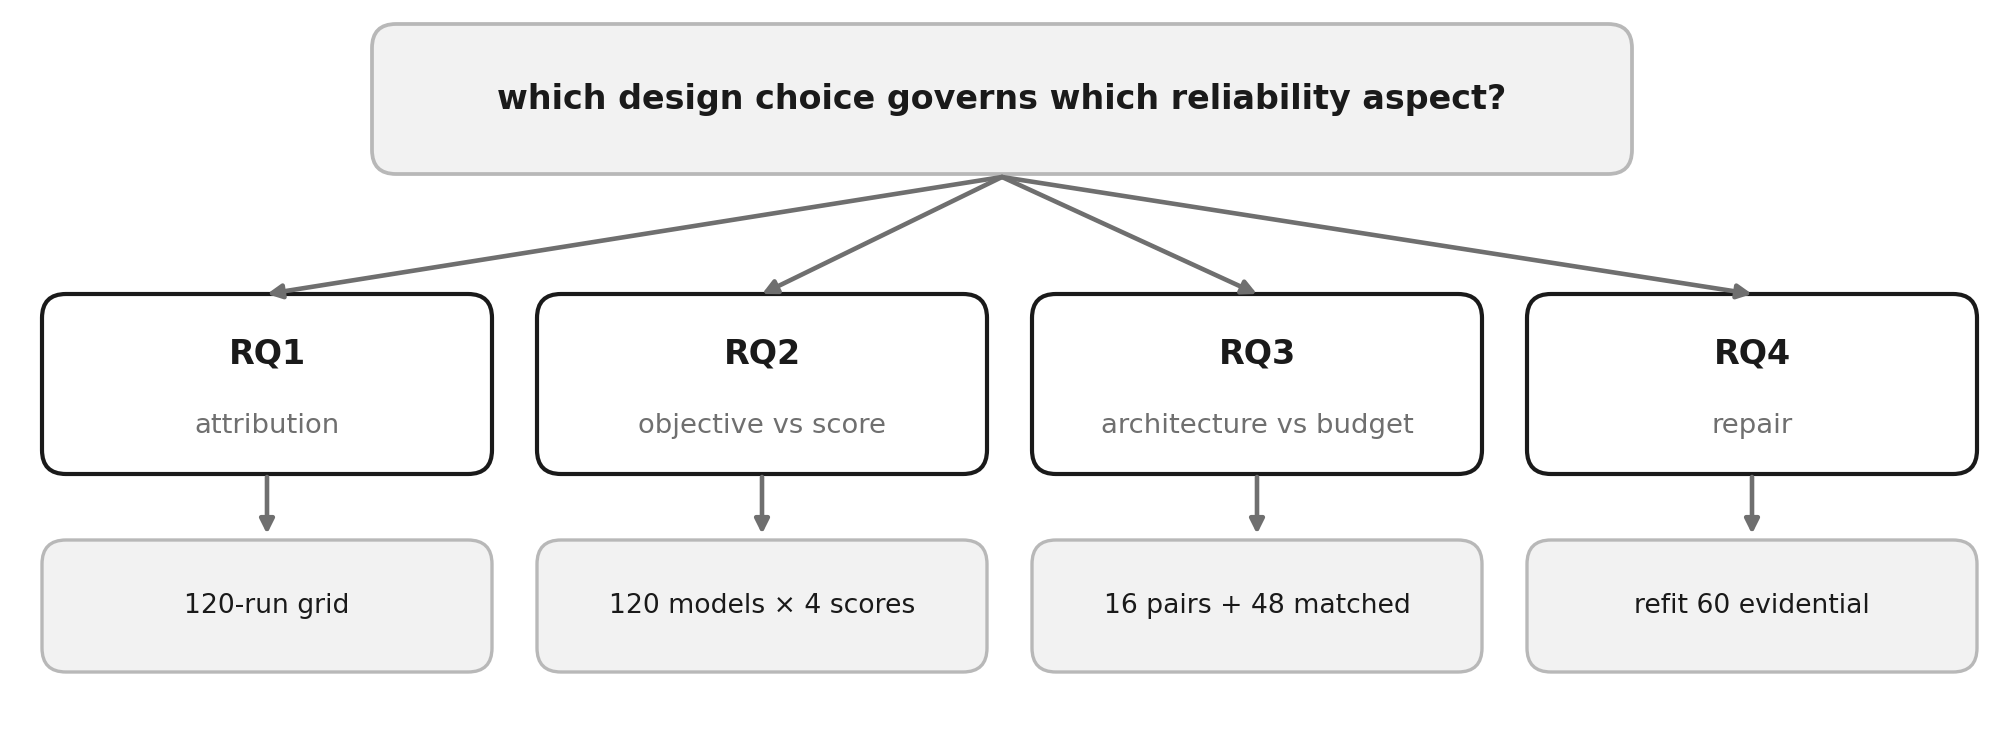
\includegraphics[width=0.95\textwidth]{F1_research_roadmap.png}
\caption{The four research questions are instances of one question: which design choice governs which
reliability aspect.}
\label{fig:roadmap}
\end{figure}

\section{Research Challenges}

\paragraph{Confounded comparisons.} Two adapters rarely differ in one property only. In our grid the
bottleneck adapter is the larger adapter on ResNet-18 but the smaller one on MobileNetV3-Small, so
adapter size and backbone always change together. Separating them required a dedicated matched-budget
experiment (\cref{sec:rq3}).

\paragraph{A fragile evidential head.} Our first evidential model did not train at all. Softplus was
applied directly to negative squared-distance logits of magnitude in the hundreds, so every class
received essentially zero evidence and the gradients vanished. Switching to scaled cosine logits and
adding a learnable scale and bias before the softplus (\cref{sec:readouts}) fixed this, and those two
parameters later became the subject of RQ4.

\paragraph{Noisy few-shot estimates.} With one or five support images, a single episode says little.
Every number in this thesis is averaged over the same 600 fixed test episodes and over three training
seeds.

\section{Contributions}

\begin{enumerate}
\item \textbf{A controlled, reliability-complete comparison.} A balanced 120-run grid (40
configurations $\times$ 3 seeds) of frozen lightweight CNNs with small adapters, evaluated for accuracy,
macro-F1, calibration (ECE, Brier) and OOD detection (AUROC, FPR@95) on the same 600 test episodes.
\item \textbf{A variance decomposition (RQ1).} Shot count explains about 76\% of accuracy variance and
head type about 83\% of calibration variance, while the head explains only 0.2\% of accuracy variance.
\item \textbf{A separation of training objective from scoring rule (RQ2).} Scoring every model with
every score shows that the score explains 42.7\% of far-OOD variance against 0.17\% for the objective.
The energy score works almost as well on evidential-trained logits as on softmax-trained ones.
\item \textbf{A pre-registered matched-budget experiment (RQ3).} At equal parameter budget, accuracy and
near-OOD detection still follow adapter architecture, whereas the calibration gap follows the backbone
rather than the budget.
\item \textbf{A measured post-hoc repair (RQ4).} Refitting two parameters improves evidential
calibration in 60 of 60 models; we report both what it repairs and what it costs in OOD ranking.
\end{enumerate}

\section{Thesis Organization}

\Cref{ch:related} reviews related work and positions the thesis. \Cref{ch:data} describes the datasets,
backbones, episodic protocol and metrics. \Cref{ch:method} describes the system and the experimental
design. \Cref{ch:results} answers the four research questions and discusses deployment cost,
positioning and limitations. \Cref{ch:conclusion} concludes. \Cref{app:tables} contains the full result
tables.

\chapter{Related Work}
\label{ch:related}

This thesis draws on five lines of work that are usually studied separately: parameter-efficient
fine-tuning, evidential and Bayesian uncertainty, calibration, out-of-distribution detection, and
few-shot learning. We review each with an eye on the design decision it informs, then position the
thesis against the closest prior work.

\section{Parameter-Efficient Fine-Tuning}

Houlsby et al.~\cite{houlsby2019adapters} introduced adapters for transformers: small bottleneck modules
(a down-projection, a non-linearity and an up-projection) inserted into a frozen network, with only the
bottlenecks trained. LoRA~\cite{hu2022lora} instead learns a low-rank update to an existing weight
matrix, $W = W_0 + BA$. Because the update can be merged into $W_0$ after training, LoRA adds no
inference latency. He et al.~\cite{he2022unified} show that adapters, LoRA and prefix tuning can be
written as variants of one update, differing in where the update is applied and whether it runs in
series with or in parallel to the frozen layer. We use their serial/parallel vocabulary. In vision, the
same ideas were carried over to Vision Transformers, for example visual prompt tuning~\cite{jia2022vpt}
and AdaptFormer~\cite{chen2022adaptformer}; a recent survey~\cite{xin2024peftsurvey} covers this body of
work and does not discuss calibration or OOD detection.

Work on CNNs is thinner. Conv-Adapter~\cite{chen2024convadapter} studies adapter design for ConvNets
and argues that adapters should respect the spatial structure of convolutional features, preferring
depth-wise $k \times k$ adapters to purely $1 \times 1$ ones. Convolutional variants of LoRA have been
proposed for domain adaptation~\cite{aleem2024convlora} and for the Segment Anything
model~\cite{zhong2024convlora}. Closest to our setting, Task-Specific Adapters (TSA)~\cite{li2022tsa}
attach adapters to a frozen ResNet-18 for cross-domain few-shot learning, classify with a
parameter-free nearest-centroid head, and find that parallel (residual) adapters outperform serial ones.
FiT~\cite{shysheya2023fit} adapts frozen CNN backbones with FiLM layers for few-shot transfer. For
vision-language models, CLIP-Adapter~\cite{gao2024clipadapter} and Tip-Adapter~\cite{zhang2022tipadapter}
attach small adapters to a frozen CLIP encoder. None of these works measures calibration and OOD
detection together with the adapter choice.

\section{Evidential and Bayesian Uncertainty}

A standard softmax classifier outputs one probability vector and has no way of saying ``none of the
above''. Bayesian methods place a distribution over weights, and deep
ensembles~\cite{lakshminarayanan2017ensembles} approximate this by training several networks, at a
multiplied training and inference cost. Evidential deep learning~\cite{sensoy2018edl} instead places a
distribution over the output. The network produces non-negative evidence $e_k$ for each class, which
defines a Dirichlet with parameters $\alpha_k = e_k + 1$, total strength $S = \sum_k \alpha_k$,
expected probabilities $\hat p_k = \alpha_k / S$ and vacuity $u = K/S$. Little evidence for any class
gives small $S$ and high vacuity, and all of this is available from a single deterministic forward
pass. Prior networks~\cite{malinin2018prior} use a related Dirichlet parameterisation but need OOD data
during training. Gao et al.~\cite{gao2024edlsurvey} survey the evidential literature, and Chen et
al.~\cite{chen2024redl} show that two standard ingredients of the EDL loss, the fixed ``$+1$'' prior and
the variance term, are not essential and can hurt calibration. Our evidential loss drops the variance
term accordingly (\cref{sec:edl-loss}).

The evidential approach has known weaknesses. Bengs et al.~\cite{bengs2022pitfalls} show that
uncertainty estimators trained by loss minimisation, standard EDL objectives included, need not behave
like faithful epistemic uncertainty, and Shen et al.~\cite{shen2024mirage} question how much of EDL's
apparent uncertainty quality is real. Hayta et al.~\cite{hayta2026plugin} show that the softmax
classifier is a special case of an evidential classifier under a family of plug-in losses, which helps
explain one of our RQ2 findings.

Bayesian ideas have also been combined with PEFT. Laplace-LoRA~\cite{yang2024laplacelora} fits a
post-hoc Laplace approximation over LoRA weights, and BLoB~\cite{wang2024blob} learns a variational
posterior over LoRA during training; both target large language models. In vision, Pandey et
al.~\cite{pandey2024bayesianpeft} find that PEFT-adapted vision foundation models are underconfident in
few-shot settings and propose a Bayesian PEFT framework with base-rate adjustment and an evidential
ensemble. BayesAdapter~\cite{moralesalvarez2026bayesadapter} learns a probability distribution over the
parameters of a CLIP adapter instead of a point estimate and reports better calibration and selective
classification. Bayesian Evidential Learning
(BEL)~\cite{linghu2022bel} brings evidential uncertainty to few-shot classification; on miniImageNet
5-shot it lowers the ECE of a Meta-Baseline model with a Conv-4 backbone from 14.69\% to 3.59\%. Its
backbone is meta-trained end to end, unlike ours.

\section{Calibration}

Guo et al.~\cite{guo2017calibration} showed that modern deep networks are overconfident, popularised
the expected calibration error (ECE) as a summary measure, and proposed temperature scaling: dividing
the logits by one scalar fitted on held-out data by minimising the negative log-likelihood. Because it
is a monotone rescaling, temperature scaling never changes the predicted class. Minderer et
al.~\cite{minderer2021revisiting} revisit calibration for newer architectures and find that model family
matters a great deal, and Tao et al.~\cite{tao2024benchmark} study calibration across a large space of
architectures. Neither decomposes calibration variance across design factors the way RQ1 does. Dirichlet
calibration~\cite{kull2019dirichlet} uses the word ``Dirichlet'' in a different sense: it is a post-hoc
calibration map for softmax outputs and is unrelated to evidential Dirichlet evidence. More flexible
accuracy-preserving calibrators also exist for softmax classifiers~\cite{zhao2026invlt}. For evidential
models, recent fixes change the model or its training, for example density-informed
pseudo-counts~\cite{carlotti2026dipedl} or a self-calibrated evidence-strength head~\cite{turacan2026invascal};
neither is a small post-hoc refit of the kind studied in RQ4.

\section{Out-of-Distribution Detection}

Hendrycks and Gimpel~\cite{hendrycks2017baseline} proposed the maximum softmax probability (MSP) as a
baseline OOD score and established AUROC as the standard evaluation. Liu et al.~\cite{liu2020energy}
proposed the energy score, the log-sum-exp of the logits, which needs no retraining and separates OOD
inputs better than MSP. OpenOOD~\cite{yang2022openood,zhang2024openood15} standardised the distinction
between far-OOD (semantically unrelated data, such as digits for an animal classifier) and near-OOD
(related but unseen classes) that we follow. McNamara~\cite{mcnamara2026vacuity} shows that
vacuity-based AUROC can be inflated when the in-distribution and OOD evaluations use different numbers
of classes; in our protocol every OOD image is scored by the same 5-way episode head, so this artefact
does not arise.

Two recent studies are close to RQ2. Gen{\c{c}} et al.~\cite{genc2026objectives} compare training
objectives for OOD detection and note that, in prior work, each objective tends to be evaluated with
the confidence measure natural to its output space, so objective and score are not fully separated.
Their objectives do not include an evidential one, and they do not study frozen backbones or episodic
evaluation. Krumpl et al.~\cite{krumpl2026onemodel} cross 56 ImageNet-trained ResNet-50 models with 21
post-hoc detectors on 8 OOD sets and find a strong dependence between training strategy and detector.
We run a smaller crossing of the same kind, with evidential models included.

\section{Few-Shot Learning}

Few-shot classification is usually evaluated with $N$-way $K$-shot episodes~\cite{vinyals2016matching}:
each episode samples $N$ classes, $K$ labelled support images per class, and a set of query images to
classify. We use the MiniImageNet split of Ravi and Larochelle~\cite{ravi2017optimization} and the
CIFAR-FS split of Bertinetto et al.~\cite{bertinetto2019r2d2}. Prototypical networks~\cite{snell2017protonet}
classify a query by its distance to each class prototype, the mean embedding of the class's support
images, and need no trainable classifier. Chen et al.~\cite{chen2019closer} show that simple baselines
with a cosine-similarity classifier are strong few-shot competitors. MetaOptNet~\cite{lee2019metaoptnet}
is a representative method trained from scratch on the base classes, while P>M>F~\cite{hu2022pmf} shows
how much large-scale pretraining (for example DINO~\cite{caron2021dino}) adds when the whole backbone is
then meta-trained and fine-tuned.

\section{Backbones for Edge Deployment}

We use ResNet-18~\cite{he2016resnet} and MobileNetV3-Small~\cite{howard2019mobilenetv3}, both
pretrained on ImageNet. They were chosen because they are realistic for constrained hardware, not for
peak accuracy. A recent survey of tiny machine learning~\cite{somvanshi2025tinydl} describes the memory
and compute limits of such hardware and the continued role of compact CNNs there.

\section{Positioning}

\Cref{tab:gap} compares this thesis with the three closest pieces of prior work. Each covers some of
the four properties we study, but none covers all of them. In addition, we separate two pairs of factors
that published comparisons usually change together: the training objective versus the OOD scoring rule
(RQ2), and adapter architecture versus parameter budget (RQ3).

\begin{table}[H]
\centering
\caption{The research gap. Each close prior work covers some, but not all, of the four properties
studied here.}
\label{tab:gap}
\begin{adjustbox}{max width=\textwidth}
\begin{tabular}{@{}lcccc@{}}
\toprule
& Frozen lightweight CNN & Parameter-efficient adapter & Calibration & OOD detection \\
\midrule
TSA~\cite{li2022tsa} & \cmark & \cmark & \xmark & \xmark \\
BEL~\cite{linghu2022bel} & \xmark\ (meta-trained) & \xmark & \cmark & \xmark \\
BayesAdapter~\cite{moralesalvarez2026bayesadapter} & \xmark\ (frozen CLIP) & \cmark & \cmark & \xmark \\
This work & \cmark & \cmark & \cmark & \cmark \\
\bottomrule
\end{tabular}
\end{adjustbox}
\end{table}

\chapter{Datasets, Backbones and Evaluation Protocol}
\label{ch:data}

This chapter fixes the experimental ground: the datasets and their splits, the OOD sets, the two
backbones, the episodic protocol, and the metrics.

\section{Datasets}
\label{sec:datasets}

\subsection{In-distribution datasets}

Both datasets use the standard 64/16/20 class split: 64 classes for training the adapter, 16 for
validation and 20 held out for testing. The three groups of classes are disjoint, so test accuracy
measures generalisation to classes the adapter has never seen.

\begin{itemize}
\item \textbf{CIFAR-FS}~\cite{bertinetto2019r2d2}: the 100 classes of CIFAR-100~\cite{krizhevsky2009cifar}
($32 \times 32$ images), split 64/16/20.
\item \textbf{MiniImageNet}~\cite{vinyals2016matching}: 100 ImageNet classes stored at $84 \times 84$,
with the split of Ravi and Larochelle~\cite{ravi2017optimization}.
\end{itemize}

The backbones were pretrained at $224 \times 224$, so every image is resized to $224 \times 224$ and
normalised with the ImageNet mean and standard deviation. No data augmentation is used. The class splits
are stored as fixed files and never regenerated.

\subsection{Out-of-distribution sets}

Each in-distribution dataset is evaluated against four OOD sets of 500 images each, drawn once with a
fixed seed and preprocessed in the same way:

\begin{itemize}
\item \textbf{SVHN}~\cite{netzer2011svhn} (far-OOD): street-view house-number digits from the SVHN test
set, unrelated to the natural-image classes.
\item \textbf{Gaussian noise} (far-OOD): images of independent standard normal noise, the simplest
possible OOD input.
\item \textbf{Held-out classes} (near-OOD): 500 images from the 16 validation classes of the same
dataset, i.e.\ held-out CIFAR-100 classes for CIFAR-FS and held-out MiniImageNet classes for
MiniImageNet. These share the visual domain of the in-distribution data but are never test classes.
\item \textbf{TinyImageNet}~\cite{le2015tinyimagenet} (near-OOD): images from the TinyImageNet training
partition. For MiniImageNet, the 25 TinyImageNet classes that also appear among MiniImageNet's 100
classes are removed first, so the pool cannot contain in-distribution classes.
\end{itemize}

The held-out near-OOD classes are the same 16 validation classes that are used for early stopping,
temperature scaling and the RQ4 refit. They are disjoint from the test classes, but model selection has
already seen them, which may make this pool somewhat easier than a truly unseen one. TinyImageNet has no
such overlap, and for that reason RQ1 uses TinyImageNet as its near-OOD outcome (\cref{sec:limits}).

\section{Backbones}

Two ImageNet-pretrained backbones are used, and both stay frozen during adaptation (except in the full
fine-tuning baseline). In both cases the classification layer is removed and the globally pooled feature
vector is used as the image embedding.

\begin{itemize}
\item \textbf{ResNet-18}~\cite{he2016resnet}: 11.18M parameters without the classifier and a
512-dimensional embedding.
\item \textbf{MobileNetV3-Small}~\cite{howard2019mobilenetv3}: 0.93M parameters without the classifier
and a 576-dimensional embedding (the last convolutional feature before the classifier's expansion
layer). The full torchvision model, including its classifier, has about 2.5M parameters.
\end{itemize}

The backbones' BatchNorm statistics are also kept fixed during training, so the frozen part of the
network computes exactly what it computed after ImageNet pretraining.

\section{Episodic Protocol}
\label{sec:protocol}

All experiments use 5-way $K$-shot episodes (\cref{fig:episode}).

\begin{figure}[H]
\centering
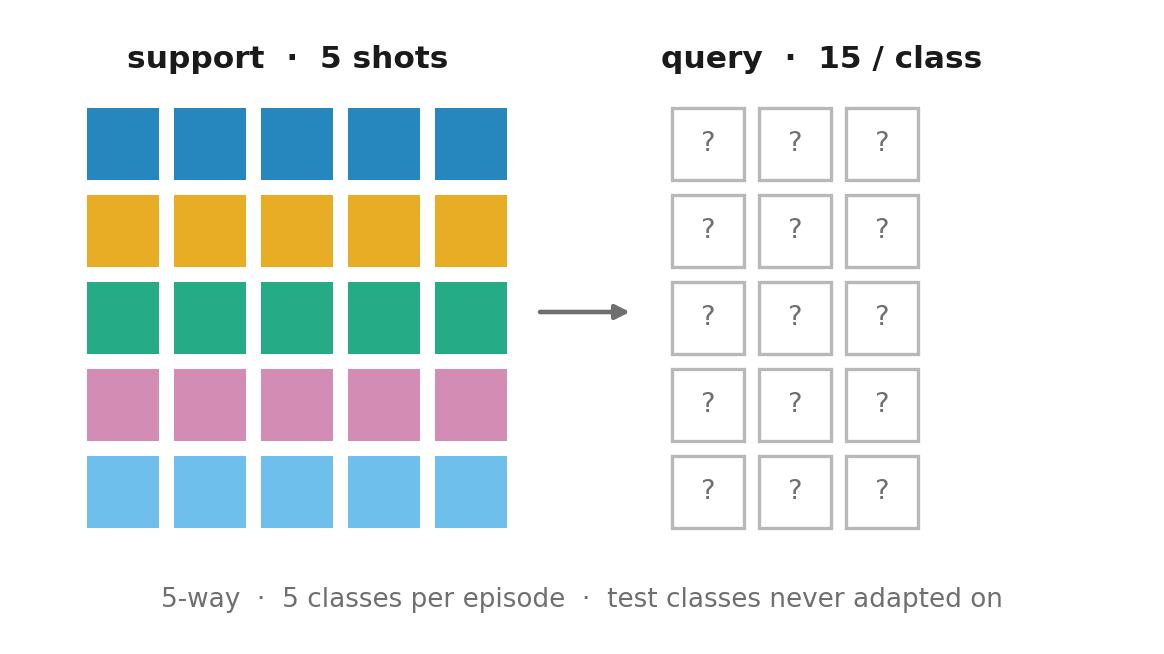
\includegraphics[width=0.6\textwidth]{F2_few_shot_episode_compact.png}
\caption{One 5-way 5-shot episode: five labelled support images per class, and fifteen query images per
class to classify. Test episodes draw their classes only from the 20 test classes.}
\label{fig:episode}
\end{figure}

\begin{itemize}
\item \textbf{Task format.} Each episode samples 5 classes, $K \in \{1, 5\}$ support images per class
and 15 query images per class, giving 75 queries per episode.
\item \textbf{Test episodes.} 600 test episodes are generated from fixed seeds (0--599), stored in the
repository and never changed, so every reported number is computed on exactly the same episodes.
\item \textbf{Validation episodes.} 100 episodes from the validation classes, with their own fixed
seeds (10000--10099), are used for early stopping and for every quantity fitted after training
(temperature scaling and the RQ4 refit). The test episodes are used only for final reporting.
\item \textbf{Training seeds.} Each configuration is trained three times, with seeds 42, 43 and 44. The
stream of training episodes is the same for all seeds, so the seed changes only the random
initialisation of the adapter. We report the mean over the three seeds and use the spread across seeds
to judge whether two configurations really differ.
\end{itemize}

\section{Evaluation Metrics}
\label{sec:metrics}

\subsection{Accuracy and macro-F1}

Top-1 accuracy and macro-averaged F1 are computed per episode and averaged over the 600 test episodes.
In balanced 5-way episodes the two track each other closely.

\subsection{Calibration}

The expected calibration error groups predictions into $M = 15$ equal-width confidence bins
$B_1, \dots, B_M$ and averages the gap between each bin's accuracy and its mean confidence, weighted by
the bin's share of the $n$ predictions:
\begin{equation}
\mathrm{ECE} = \sum_{m=1}^{M} \frac{|B_m|}{n} \,\bigl|\mathrm{acc}(B_m) - \mathrm{conf}(B_m)\bigr| .
\label{eq:ece}
\end{equation}
Our main calibration number is the \emph{pooled} ECE, computed over all 45{,}000 query predictions of
the 600 episodes together. We also report the per-episode ECE (computed on each episode's 75 queries and
then averaged, which is noisier) and the multi-class Brier score,
\begin{equation}
\mathrm{BS} = \frac{1}{n}\sum_{i=1}^{n}\sum_{k=1}^{K}\bigl(\hat p_{i,k} - y_{i,k}\bigr)^2 ,
\end{equation}
a proper scoring rule that uses the whole predicted distribution. For softmax models we also report ECE
after temperature scaling~\cite{guo2017calibration}, with the temperature fitted on the validation
episodes.

\subsection{OOD detection}

In each test episode the 75 in-distribution queries and the 500 images of an OOD set are scored against
that episode's five prototypes with a chosen uncertainty score (\cref{sec:scores}). The area under the
ROC curve (AUROC) measures how well the score separates the two groups: it is the probability that a
randomly chosen OOD image is rated more uncertain than a randomly chosen in-distribution query. We also
report the false-positive rate at 95\% true-positive rate (FPR@95), the fraction of OOD images still
accepted when the threshold keeps 95\% of the in-distribution queries. Both are averaged over the 600
episodes. Higher AUROC and lower FPR@95 are better.

\subsection{Efficiency}

We report the number of trainable parameters and the inference latency per image, measured on a single
CPU thread (median over repeated runs) as a proxy for constrained hardware.

\chapter{Methodology}
\label{ch:method}

\section{Overview}

The system has three parts (\cref{fig:pipeline}). A frozen ImageNet-pretrained CNN turns each image
into an embedding. A small trainable adapter inside the backbone changes those embeddings; it is the
only part that is trained, apart from two scalars in the evidential head. A parameter-free prototype
head then classifies each query by its similarity to the class prototypes of the current episode, and
the resulting logits are read either as a softmax or as Dirichlet evidence.

\begin{figure}[H]
\centering
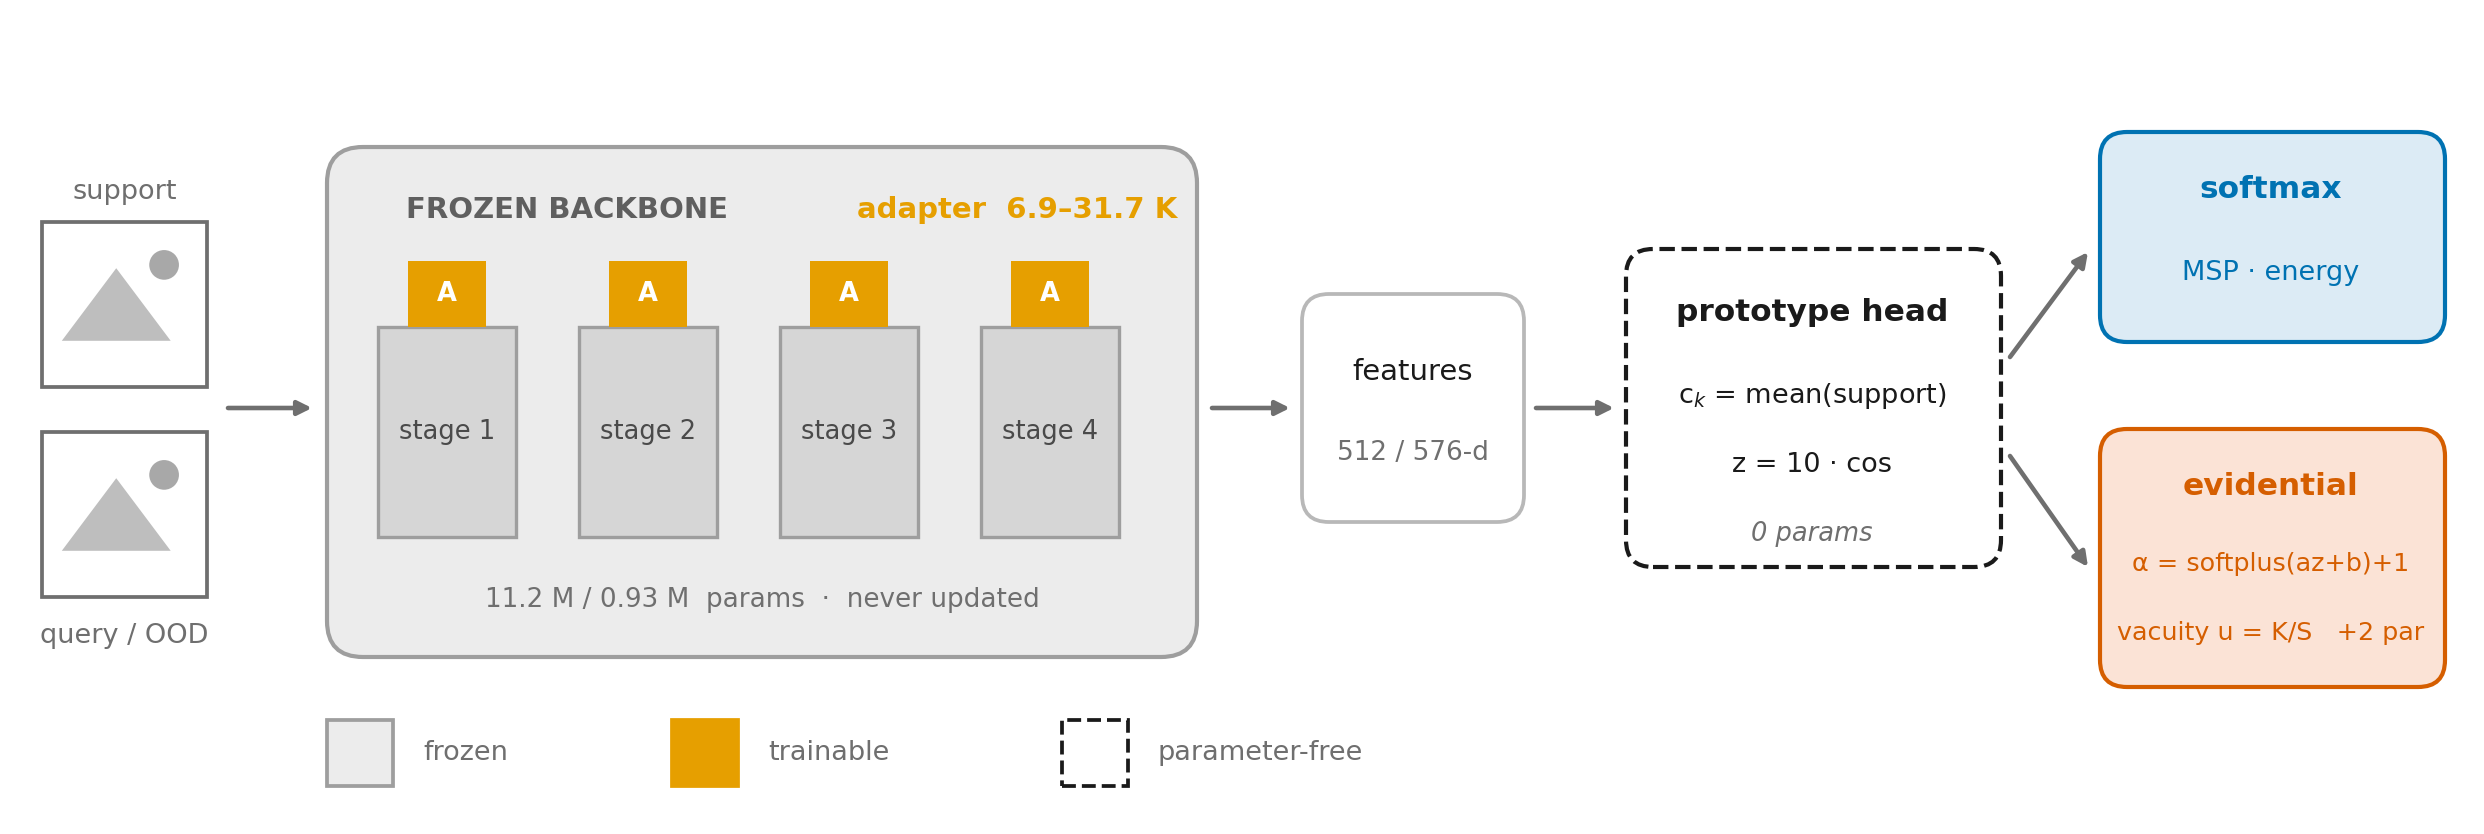
\includegraphics[width=\textwidth]{F4_architecture_pipeline.png}
\caption{The pipeline. Support and query images pass through the frozen backbone with a small trainable
adapter. The features feed a parameter-free prototype head whose logits are read as softmax
probabilities or as evidential (Dirichlet) evidence. Only the adapter and, for the evidential head, two
evidence parameters are trained.}
\label{fig:pipeline}
\end{figure}

\section{Adapters}
\label{sec:adapters}

Two adapter designs form the main comparison (\cref{fig:adapters}). Both are initialised so that the
adapted network starts out identical to the pretrained one.

\begin{figure}[H]
\centering
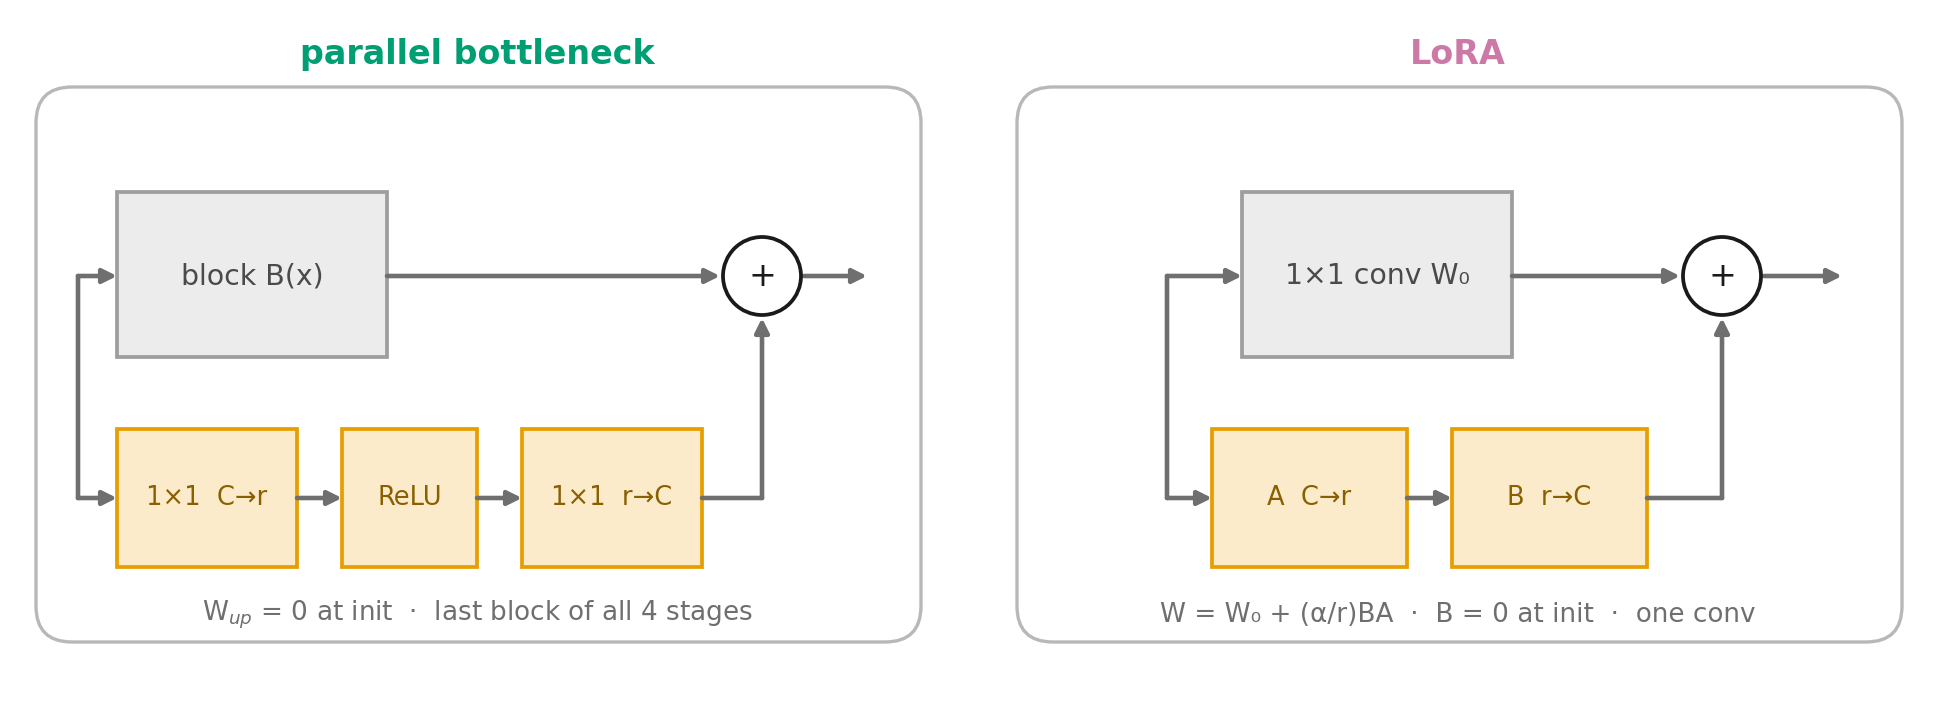
\includegraphics[width=0.95\textwidth]{F5a_adapter_zooms.png}
\caption{The two adapter designs. Left: the parallel bottleneck, a side branch added at the last block
of each of the four stages. Right: LoRA, a low-rank update inside one frozen $1\times1$ convolution.}
\label{fig:adapters}
\end{figure}

\paragraph{Parallel bottleneck adapter.} Following Houlsby et al.~\cite{houlsby2019adapters}, the
adapter is a down-projection to $r$ channels, a ReLU and an up-projection back to $C$ channels:
\begin{equation}
g(x) = W_{\text{up}}\, \mathrm{ReLU}(W_{\text{down}} x), \qquad W_{\text{down}} \in \mathbb{R}^{r \times C},\;
W_{\text{up}} \in \mathbb{R}^{C \times r}.
\end{equation}
Both projections are $1 \times 1$ convolutions with biases, applied at every spatial position, and
$W_{\text{up}}$ starts at zero. In the terminology of He et al.~\cite{he2022unified} the adapter is
\emph{parallel}: for the last block $B$ of each stage, the output becomes $B(x) + g(x)$, so the adapter
reads the block's input and its output is added to the block's output. One adapter is placed in each of
the four stages of ResNet-18, and in the last residual block of each of the four channel widths of
MobileNetV3-Small. We use $r = 16$. With biases, one stage costs $33C + 16$ parameters, which gives
31,744 parameters for ResNet-18 (stage widths 64, 128, 256, 512) and 6,928 for MobileNetV3-Small (stage
widths 24, 40, 48, 96). Because $1\times1$ convolutions mix channels but not neighbouring positions,
this adapter does not follow Conv-Adapter's advice to use spatial kernels~\cite{chen2024convadapter}; we
kept the simpler form so that the same adapter could be used unchanged on both backbones.

\paragraph{LoRA.} Following Hu et al.~\cite{hu2022lora}, LoRA adds a low-rank update to one frozen
$1 \times 1$ convolution:
\begin{equation}
W = W_0 + \tfrac{\alpha}{r}\, B A, \qquad A \in \mathbb{R}^{r \times C_{\text{in}}},\; B \in
\mathbb{R}^{C_{\text{out}} \times r},
\end{equation}
with $B$ initialised to zero, $r = 16$ and $\alpha = r$. On ResNet-18 the target is the $1\times1$
downsampling convolution at the start of the last stage ($256 \to 512$ channels), giving
$16 \times (256 + 512) = 12{,}288$ parameters. On MobileNetV3-Small it is the $1\times1$ projection
convolution of the deepest block ($576 \to 96$), giving 10,752 parameters. Applying LoRA to
convolutions follows earlier convolutional LoRA work~\cite{aleem2024convlora,zhong2024convlora}.

\paragraph{Baselines.} Two reference points are trained on ResNet-18 and CIFAR-FS only. \emph{Full
fine-tuning} unfreezes all 11.18M backbone parameters (learning rate $10^{-5}$, weight decay $10^{-4}$).
The \emph{linear probe} trains no backbone or adapter parameters: frozen features go straight to the
prototype head, so it has zero trainable parameters with the softmax head and only the two evidence
parameters with the evidential head.

\section{The Prototype Head}
\label{sec:head}

Classification uses a prototypical-network head~\cite{snell2017protonet}. For each of the $N$ classes of
an episode, the prototype is the mean embedding of its $K$ support images,
\begin{equation}
c_n = \frac{1}{K}\sum_{i \in \mathcal{S}_n} f_\theta(x_i),
\end{equation}
where $f_\theta$ is the frozen backbone with its adapter. A query $x$ receives one logit per class, its
scaled cosine similarity to that class's prototype:
\begin{equation}
z_n(x) = \tau \, \frac{f_\theta(x) \cdot c_n}{\lVert f_\theta(x)\rVert\, \lVert c_n \rVert}, \qquad \tau = 10 .
\label{eq:logits}
\end{equation}
The head has no trainable weights. This matters because the test classes are disjoint from the training
classes: a linear classifier trained on the 64 training classes has no outputs for the 20 test classes,
whereas prototypes can be computed for any class from its support images. At test time no gradient steps
are taken at all.

We use cosine similarity rather than the negative squared Euclidean distance of the original prototypical
networks for two reasons. Raw squared distances between ResNet-18 features are large negative numbers,
which is exactly what made our first evidential head collapse (\cref{sec:readouts}); cosine logits are
bounded in $[-\tau, \tau]$. Cosine classifiers are also a standard few-shot baseline~\cite{chen2019closer}.
The scale $\tau = 10$ is needed because unscaled cosine logits lie in $[-1, 1]$, which would cap softmax
confidence at about 65\% even for a perfect match. We did not rerun the Euclidean variant under the final
training recipe, so we cannot say what accuracy, if any, this choice costs.

\section{Two Readouts of the Same Logits}
\label{sec:readouts}

The prototype head always produces the same kind of logits $z$; the head type decides how they are read
(\cref{fig:readouts}, \cref{tab:readouts}).

\begin{figure}[H]
\centering
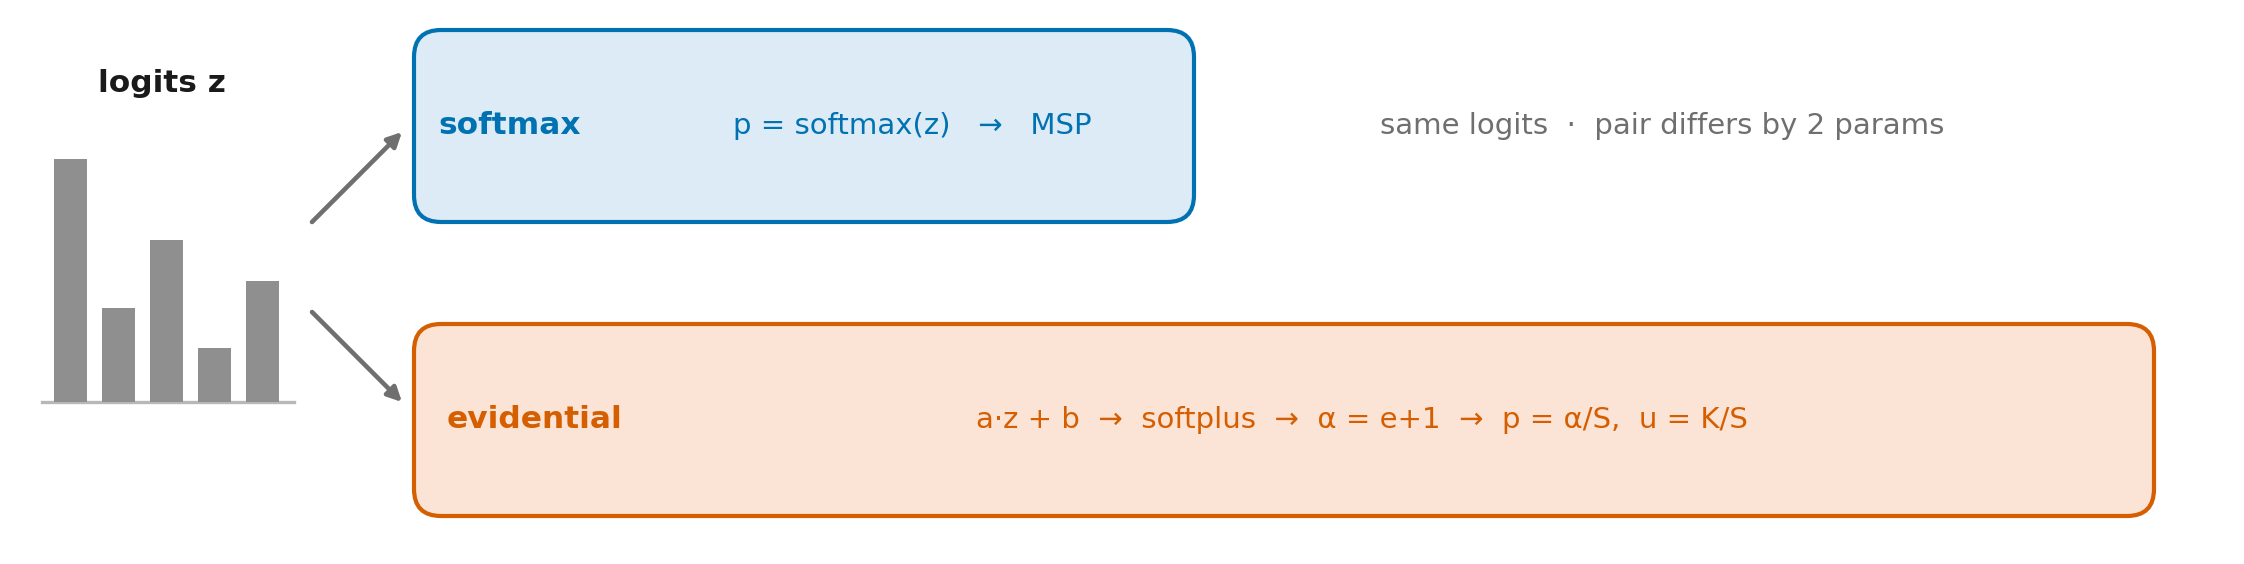
\includegraphics[width=0.95\textwidth]{F6a_head_two_readouts.png}
\caption{One set of logits, read two ways: as softmax probabilities, or as Dirichlet evidence with a
vacuity score. The two readouts differ by two parameters.}
\label{fig:readouts}
\end{figure}

\paragraph{Softmax.} The probabilities are $\hat p = \mathrm{softmax}(z)$ and the predicted class is the
arg-max.

\paragraph{Evidential.} Following Sensoy et al.~\cite{sensoy2018edl}, the logits are mapped to
non-negative evidence, which defines a Dirichlet distribution:
\begin{equation}
e_n = \mathrm{softplus}(a\, z_n + b), \quad \alpha_n = e_n + 1, \quad S = \sum_{n} \alpha_n, \quad
\hat p_n = \frac{\alpha_n}{S}, \quad u = \frac{K}{S}.
\label{eq:evidence}
\end{equation}
The vacuity $u$ is close to 1 when the model has almost no evidence for any class and close to 0 when it
has a lot, regardless of which class the evidence favours. The scale $a$ and bias $b$ are the only
parameters this readout adds. They are learned together with the adapter, start at $a = 2$, $b = -6$,
and $a$ is kept positive so that a higher similarity always produces more evidence.

These two parameters exist because of a failure we hit early in the project. In the first version,
softplus was applied directly to squared-distance logits, which are of the order of $-700$ for
ResNet-18 features. Softplus of such values is essentially zero, so every class received no evidence,
the Dirichlet was uniform, accuracy stayed at chance and the gradients vanished. The bias $b$ moves the
logits into the range where softplus responds, and the scale $a$ sets how quickly evidence grows above
that point. The same evidence function is used in the training loss, in evaluation and in OOD scoring,
so the three can never disagree.

\begin{table}[H]
\centering
\caption{The two readouts. Both use the same logits (\cref{eq:logits}).}
\label{tab:readouts}
\begin{adjustbox}{max width=\textwidth}
\begin{tabular}{@{}lll@{}}
\toprule
& Softmax & Evidential (Dirichlet) \\
\midrule
Output & class probabilities & evidence $\rightarrow$ Dirichlet $\rightarrow$ probabilities \\
Native uncertainty score & maximum probability (MSP) & vacuity $u = K/S$ \\
Extra parameters & 0 & 2 (scale $a$, bias $b$) \\
\bottomrule
\end{tabular}
\end{adjustbox}
\end{table}

\section{Training}
\label{sec:training}

\subsection{Losses}
\label{sec:edl-loss}

Softmax models are trained with cross-entropy on the query predictions. Evidential models use the
squared-error loss of Sensoy et al.~\cite{sensoy2018edl} without its variance term, which Chen et
al.~\cite{chen2024redl} found unnecessary and harmful to calibration, plus the usual Kullback--Leibler
penalty on evidence for the wrong classes:
\begin{equation}
\mathcal{L} = \sum_{k=1}^{K} \bigl(y_k - \hat p_k\bigr)^2 + \lambda_t\, \mathrm{KL}\bigl[\mathrm{Dir}(\tilde\alpha)\,\Vert\,\mathrm{Dir}(\mathbf{1})\bigr],
\qquad \tilde\alpha = y + (1 - y) \odot \alpha .
\end{equation}
Removing the correct class's evidence before the KL term means only misleading evidence is pushed toward
the uniform prior. The weight $\lambda_t$ rises linearly from 0 to 0.1 over the first 1,000 training
episodes, so the penalty does not suppress evidence before the model can separate the classes.

\subsection{Episodic training}

The adapter (and, for evidential models, $a$ and $b$) is trained on episodes sampled from the 64
training classes, with the same shot count as at test time. For each episode the support and query
images pass through the backbone and adapter, prototypes are formed, query logits are computed, and the
loss is back-propagated to the trainable parameters only. We use Adam with learning rate
$5 \times 10^{-3}$ and no weight decay, 100 training episodes per epoch and at most 30 epochs. After every
epoch the model is evaluated on the 100 validation episodes; training stops when validation accuracy has
not improved for 5 epochs, and the weights from the best validation epoch are kept. One recipe is used
for every configuration and was not tuned per configuration.

\section{OOD Scoring Rules}
\label{sec:scores}

Four uncertainty scores are compared:
\begin{itemize}
\item \textbf{MSP}~\cite{hendrycks2017baseline}: the largest softmax probability, $\max_n \hat p_n$.
\item \textbf{TS-MSP}: MSP after temperature scaling~\cite{guo2017calibration}, with the temperature fitted
on the validation episodes.
\item \textbf{Energy}~\cite{liu2020energy}: $\log \sum_n \exp(z_n)$, computed directly on the raw logits.
Liu et al.\ define the energy as the negative of this quantity; we use the sign for which a higher value
means more in-distribution. It has no parameters.
\item \textbf{Vacuity}: $u = K/S$ from \cref{eq:evidence}.
\end{itemize}
In the main grid each model is scored with its native readout only: evidential models with vacuity and
softmax models with MSP, TS-MSP and energy. Any comparison between them therefore changes the training
objective and the score at the same time. RQ2 removes this confound by computing all four scores on all
120 models (\cref{sec:rq2}). Energy is computed on the same raw logits for both kinds of model. Vacuity on
a softmax-trained model needs values for $a$ and $b$, which such a model never learned, so for RQ2 we fit
them on the validation episodes with the same procedure for both training objectives (\cref{sec:refit}).

\section{Post-Hoc Refit of the Evidential Head}
\label{sec:refit}

RQ4 asks whether the evidential head's calibration can be improved after training. We keep the backbone,
adapter and prototypes fixed and refit only $a$ and $b$ on the validation-episode logits by minimising the
negative log-likelihood of $\hat p = \alpha / S$ (500 Adam steps, learning rate 0.05). This mirrors
temperature scaling~\cite{guo2017calibration}, which also fits a tiny number of parameters on held-out
data by minimising NLL. There is one important difference. Temperature scaling is a monotone rescaling
of each logit and cannot change the ranking of inputs by confidence. Vacuity, however, depends on the
evidence summed over all five classes, so changing $a$ and $b$ can reorder which images look most
unfamiliar. Whether the OOD ranking survives therefore has to be measured, and RQ4 measures it.

\section{Experimental Design}
\label{sec:design}

\subsection{The main grid}

The main grid crosses five two-level factors in a full factorial design (\cref{fig:design}):
\begin{itemize}
\item dataset: CIFAR-FS or MiniImageNet;
\item shots: 1 or 5;
\item backbone: ResNet-18 or MobileNetV3-Small;
\item adapter: parallel bottleneck or LoRA;
\item head: softmax or evidential.
\end{itemize}
This gives $2^5 = 32$ configurations. The two baselines (full fine-tuning and linear probe, with both
heads and both shot counts, on ResNet-18 and CIFAR-FS) add 8 configurations, for 40 in total. Each is
trained with 3 seeds, giving 120 runs, all evaluated on the same 600 test episodes. The baselines are not
part of the balanced factorial and are left out of the variance decomposition of RQ1.

\begin{figure}[H]
\centering
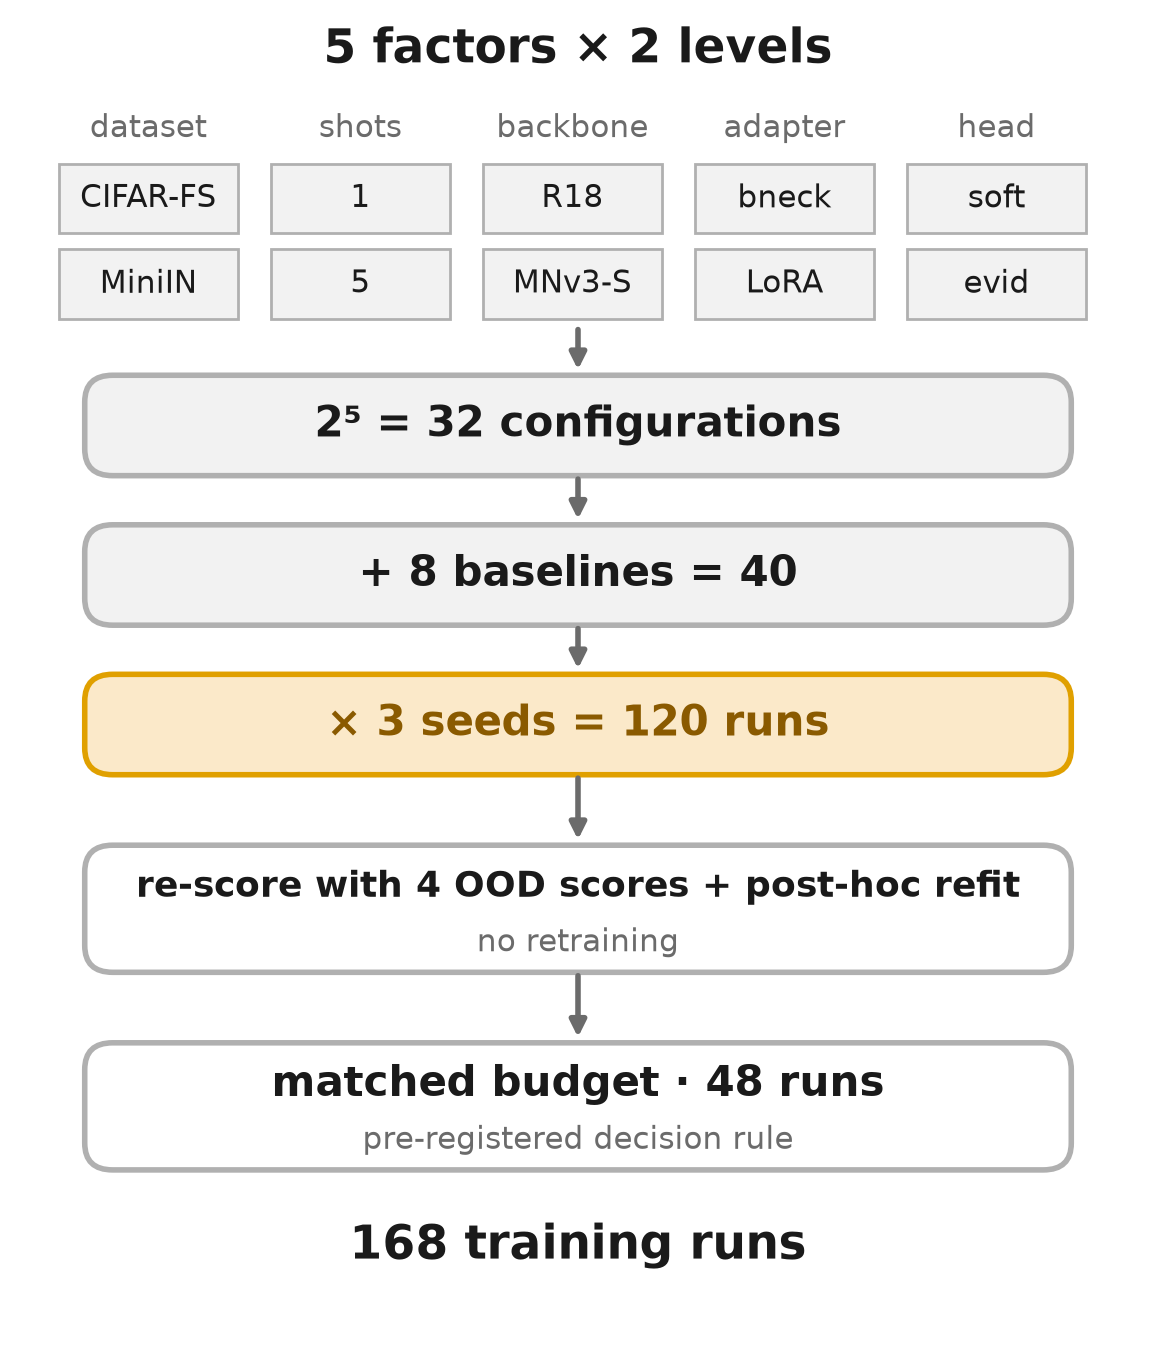
\includegraphics[width=0.55\textwidth]{F7_experimental_design_flow.png}
\caption{The experimental design: the 120-run grid, re-scored with four OOD scores and refitted post hoc
without retraining, followed by the 48-run matched-budget experiment.}
\label{fig:design}
\end{figure}

A structural feature of this grid makes RQ3 possible. Because the bottleneck adapter's size depends on
the channel widths of all four stages while LoRA's depends on one layer, the ordering of the two adapters'
sizes reverses between backbones (\cref{tab:budgets}).

\begin{table}[H]
\centering
\caption{Trainable parameters of the two adapters (softmax head; the evidential head adds 2). The size
ordering reverses between backbones.}
\label{tab:budgets}
\begin{adjustbox}{max width=\textwidth}
\begin{tabular}{@{}lrrl@{}}
\toprule
Backbone & Bottleneck & LoRA & Larger adapter \\
\midrule
ResNet-18 & 31,744 & 12,288 & bottleneck, by $2.58\times$ \\
MobileNetV3-Small & 6,928 & 10,752 & LoRA, by $1.55\times$ \\
\bottomrule
\end{tabular}
\end{adjustbox}
\end{table}

\subsection{The matched-budget experiment}
\label{sec:matched-design}

In the grid the size ordering always flips together with the backbone, so ``the larger adapter is better
calibrated'' and ``the backbone decides which adapter is better calibrated'' predict exactly the same
pattern. To tell them apart we rebuilt both adapters with the \emph{same} number of parameters within each
backbone, at two budget levels per backbone, by changing only the rank (\cref{tab:matched-budgets}). The
experiment uses MiniImageNet 5-shot, both heads (trained separately) and 3 seeds: 2 backbones $\times$ 2
levels $\times$ 2 adapters $\times$ 2 heads $\times$ 3 seeds = 48 runs, 18 of which repeat grid
configurations and reproduced the grid's numbers exactly. On MobileNetV3-Small the high level is 9.4K
rather than 10.8K because the bottleneck rank cannot exceed the 24 channels of the shallowest stage.

\begin{table}[H]
\centering
\caption{Matched budgets (softmax head). The two adapters differ in size by at most 3.1\%, against 55--158\%
in the grid.}
\label{tab:matched-budgets}
\begin{adjustbox}{max width=\textwidth}
\begin{tabular}{@{}llrrr@{}}
\toprule
Backbone & Level & Bottleneck (rank $\rightarrow$ params) & LoRA (rank $\rightarrow$ params) & Difference \\
\midrule
ResNet-18 & low & 6 $\rightarrow$ 12,504 & 16 $\rightarrow$ 12,288 & 1.8\% \\
ResNet-18 & high & 16 $\rightarrow$ 31,744 & 41 $\rightarrow$ 31,488 & 0.8\% \\
MobileNetV3-S & low & 16 $\rightarrow$ 6,928 & 10 $\rightarrow$ 6,720 & 3.1\% \\
MobileNetV3-S & high & 22 $\rightarrow$ 9,448 & 14 $\rightarrow$ 9,408 & 0.4\% \\
\bottomrule
\end{tabular}
\end{adjustbox}
\end{table}

The decision rule was written down and committed before any of these runs existed. The analysis unit is
a backbone $\times$ head cell (four cells), averaging its two budget levels. Let $\Delta$ be LoRA's ECE minus
the bottleneck's, and $\sigma$ the pooled across-seed standard deviation of the two adapters,
$\sigma = \sqrt{(s_{\text{btl}}^2 + s_{\text{LoRA}}^2)/2}$, with sample standard deviations over the
three seeds. The hypotheses and their pre-registered criteria were:
\begin{itemize}
\item \textbf{Budget:} the gap collapses once budgets are equal. The matched $|\Delta|$ is at most half of
the unmatched $|\Delta|$ (collapse ratio $\le 0.5$) and lies within $2\sigma$ of zero.
\item \textbf{Architecture:} one adapter is better calibrated on both backbones. The matched $\Delta$ has the
same sign on both backbones and exceeds $2\sigma$.
\item \textbf{Backbone:} the per-backbone signs of the grid survive at equal budget. The matched $\Delta$
keeps its unmatched sign (positive on ResNet-18, negative on MobileNetV3-Small) and exceeds $2\sigma$.
\end{itemize}
A hypothesis is supported if its rule fires in at least 3 of the 4 cells; if none does, the result is
recorded as inconclusive.

\section{Implementation}

The code is written in PyTorch and driven by configuration files, so that each experiment states only
how it differs from a shared base configuration. Every run seeds Python, NumPy and PyTorch and uses
deterministic cuDNN kernels; evaluating the same checkpoint twice gives byte-identical result files.
Training ran on NVIDIA Tesla T4 GPUs on Google Colab and Kaggle.

\chapter{Results and Discussion}
\label{ch:results}

This chapter first places the adapters against full fine-tuning and the linear probe, then answers the
four research questions in turn, and closes with deployment cost, a comparison with published few-shot
results, and the limitations of the study. All numbers are means over three training seeds, each
evaluated on the same 600 test episodes. The complete per-configuration tables are in
\cref{app:tables}.

\paragraph{A note on one corrected run.} While completing the analysis we found that one of the 120
result files (CIFAR-FS, 5-shot, MobileNetV3-Small, LoRA, evidential, seed 42) had been written by a
20-episode smoke test rather than the full 600-episode evaluation. The run was retrained and evaluated
properly; the retrained model reproduced the smoke test's numbers on the first 20 episodes exactly. All
numbers in this thesis use the corrected run. The correction changes that configuration's accuracy from
86.97\% to 87.52\% and moves the RQ1 variance shares by at most 0.7 percentage points; no conclusion
changes.

\section{Parameter Efficiency}
\label{sec:efficiency}

\Cref{fig:efficiency} compares the parallel bottleneck adapter with the two baselines on CIFAR-FS and
ResNet-18. At 5-shot, the 31,744-parameter adapter reaches 91.44\% accuracy against 90.47\% for full
fine-tuning, which trains $352\times$ more parameters (11,176,512), and 87.41\% for the linear probe,
which trains none. With the evidential head the picture is the same (91.58\% against 88.82\% and
87.41\%).

\begin{figure}[H]
\centering
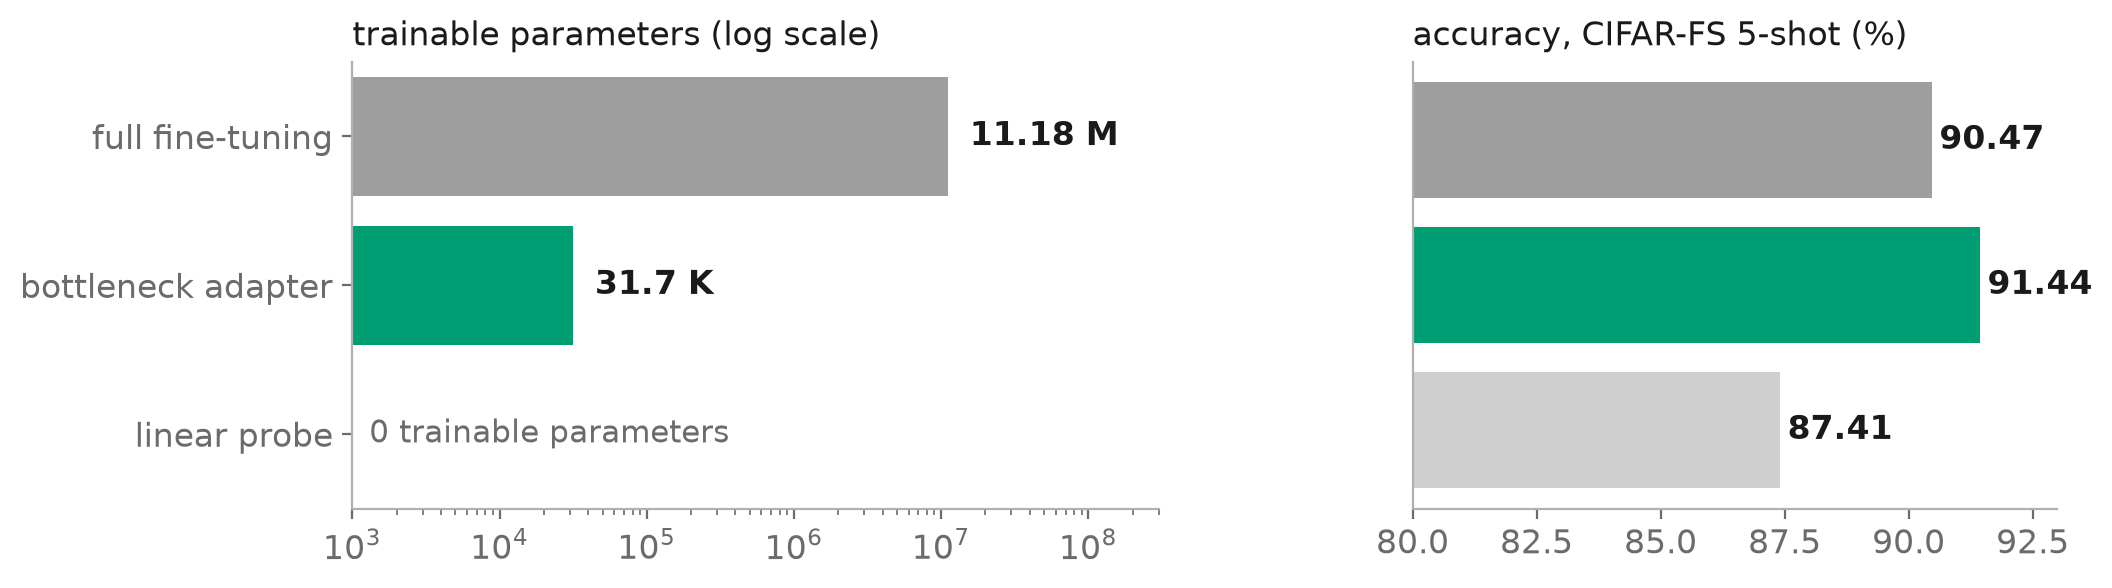
\includegraphics[width=\textwidth]{D2_parameter_efficiency_bars.png}
\caption{Trainable parameters (left, log scale) and accuracy (right) of full fine-tuning, the parallel
bottleneck adapter and the linear probe on CIFAR-FS 5-shot with ResNet-18 (softmax head).}
\label{fig:efficiency}
\end{figure}

Two qualifications matter. First, the advantage does not hold at 1-shot: there, full fine-tuning
reaches 81.14\% against 78.57\% for the adapter (80.36\% against 79.19\% with the evidential head). The
adapter comes close to full fine-tuning at 1-shot and beats it at 5-shot, but it does not dominate it. Second,
not every adapter beats the linear probe. At 5-shot on ResNet-18, LoRA reaches only 86.25\% (softmax) and
83.33\% (evidential), below the probe's 87.41\%. Adaptation pays off for the bottleneck adapter in every
setting, but not automatically for any adapter. The linear probe being a strong reference agrees with
Chen et al.'s observation that simple baselines are competitive in few-shot
classification~\cite{chen2019closer}.

The two baselines have no randomly initialised weights, and the training episodes do not depend on the
seed, so their three runs are identical. Comparisons against them therefore rest on one effective run.

\section{RQ1: What Explains Each Outcome?}
\label{sec:rq1}

We computed the share of variance ($\eta^2$) that each factor explains for each outcome, using all 96
runs of the balanced $2^5$ factorial (32 configurations $\times$ 3 seeds; the baselines are excluded).
Using individual runs rather than seed means keeps a genuine residual term. For OOD detection we use
SVHN as the far-OOD outcome and TinyImageNet as the near-OOD outcome, because TinyImageNet does not share
classes with the validation split.

\begin{table}[H]
\centering
\caption{Share of variance explained by each factor ($\eta^2$, \%), 96 runs. Bold marks the dominant
factor where one exists.}
\label{tab:eta}
\begin{adjustbox}{max width=\textwidth}
\begin{tabular}{@{}lrrrrrr@{}}
\toprule
Outcome & Dataset & Shots & Backbone & Adapter & Head & Residual \\
\midrule
Accuracy & 1.69 & \textbf{76.31} & 3.82 & 8.98 & 0.16 & 9.04 \\
ECE & 1.98 & 2.16 & 4.56 & 0.65 & \textbf{82.97} & 7.68 \\
OOD AUROC, far (SVHN) & 1.23 & 22.59 & 11.71 & 1.79 & 38.93 & 23.75 \\
OOD AUROC, near (TinyImageNet) & 1.54 & 43.30 & 0.55 & 21.68 & 21.44 & 11.49 \\
\bottomrule
\end{tabular}
\end{adjustbox}
\end{table}

\begin{figure}[H]
\centering
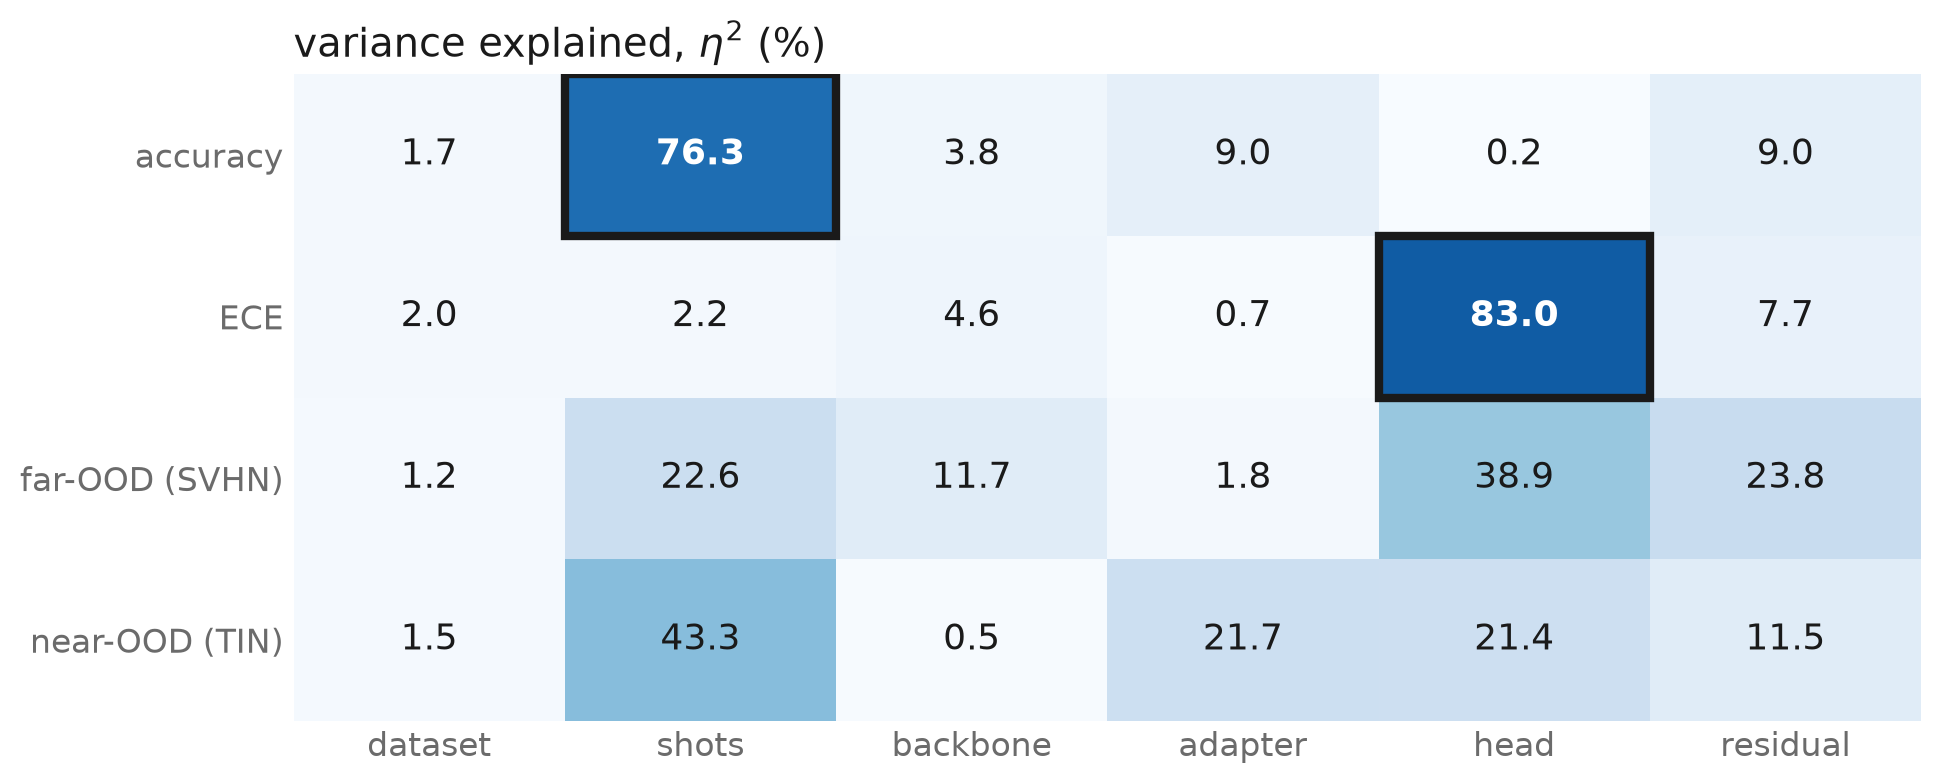
\includegraphics[width=0.9\textwidth]{F11_main_effects_heatmap.png}
\caption{The variance shares of \cref{tab:eta} as a heatmap. Accuracy is dominated by shot count and
calibration by the head; neither OOD outcome has a single dominant factor.}
\label{fig:heatmap}
\end{figure}

\paragraph{Accuracy and calibration are governed by different factors.} Shot count explains 76\% of the
variance in accuracy, and adapter type is a distant second at 9\%. The head explains 83\% of the
variance in calibration but only 0.16\% of the variance in accuracy. In practice the head changes how
confident the model is while leaving what it predicts almost untouched: across the 20 matched pairs that
differ only in the head, the evidential head is more accurate in 7 and the softmax head in 13, and no
difference exceeds 0.7 percentage points in the evidential head's favour.

\paragraph{The evidential head is worse calibrated in every case.} In all 20 matched pairs, the evidential
head has a higher pooled ECE than the softmax head, by a factor of 1.4 to 9.1, and a higher ECE than the
temperature-scaled softmax by a factor of 5.3 to 51. \Cref{tab:ece-head} shows the ResNet-18 bottleneck
configurations as an example. The gap does not shrink with more data: at 5-shot it is as large as at
1-shot. The reliability diagrams we inspected (ResNet-18 with the bottleneck adapter) show that the evidential
head is \emph{under}confident (accuracy higher than confidence in every bin), so its problem is the opposite of the overconfidence
usually reported for softmax networks.

\begin{table}[H]
\centering
\caption{Pooled ECE of the ResNet-18 bottleneck configurations. Lower is better.}
\label{tab:ece-head}
\begin{adjustbox}{max width=\textwidth}
\begin{tabular}{@{}llrrr@{}}
\toprule
Dataset & Shots & Evidential & Softmax & Softmax + temperature scaling \\
\midrule
CIFAR-FS & 1 & 0.2765 & 0.0560 & 0.0297 \\
CIFAR-FS & 5 & 0.3010 & 0.0670 & 0.0152 \\
MiniImageNet & 1 & 0.3073 & 0.1012 & 0.0073 \\
MiniImageNet & 5 & 0.2938 & 0.0850 & 0.0057 \\
\bottomrule
\end{tabular}
\end{adjustbox}
\end{table}

This negative result does not contradict the evidential literature so much as mark a boundary. BEL and
BayesAdapter report calibration improvements from evidential or Bayesian
modelling~\cite{linghu2022bel,moralesalvarez2026bayesadapter}, but with a meta-trained backbone or a
larger adaptation budget than ours. With a frozen backbone and an adapter of a few thousand parameters
we see the opposite.

\paragraph{Calibration and OOD detection are not in tension once the head is fixed.} Across the 40
configurations, the rank correlation between ECE and OOD AUROC is positive (Spearman $\rho = 0.43$ for
SVHN, $0.48$ for TinyImageNet), which would suggest that worse-calibrated models detect OOD inputs better.
Within each head the correlation drops to $0.15$/$0.20$ (evidential) and $0.26$/$0.24$ (softmax). The
apparent trade-off is almost entirely a head effect: the evidential head is both worse calibrated and,
with its native vacuity score, a better OOD detector. RQ2 shows where the second part comes from.

\paragraph{Interactions.} Adding the ten two-way interactions to the model lowers the residual from 9.0\%
to 1.3\% for accuracy and from 7.7\% to 2.0\% for ECE. For calibration the largest interaction is
backbone $\times$ adapter (3.23\%, 95\% bootstrap interval 2.49--4.05\%), while the same interaction is
negligible for accuracy (0.8\%) and for both OOD outcomes (0.2\% and 0.0\%). In other words, which adapter
calibrates better depends on the backbone, but which adapter is more accurate does not. RQ3 tests this
directly.

\section{RQ2: Training Objective or Scoring Rule?}
\label{sec:rq2}

\paragraph{The native comparison.} In the grid, each evidential model is scored with vacuity and each
softmax model with MSP, TS-MSP and energy. Comparing each evidential model's vacuity with its softmax
sibling's scores, over the two far-OOD sets and the two near-OOD sets of the 20 matched pairs (40
comparisons each), gives:

\begin{table}[H]
\centering
\caption{Vacuity (evidential models) against the softmax models' scores. Wins out of 40 comparisons per
OOD type, and mean AUROC difference.}
\label{tab:vacuity-wins}
\begin{adjustbox}{max width=\textwidth}
\begin{tabular}{@{}lrrrr@{}}
\toprule
& \multicolumn{2}{c}{Far-OOD} & \multicolumn{2}{c}{Near-OOD} \\
\cmidrule(lr){2-3}\cmidrule(lr){4-5}
Vacuity vs. & Wins & Mean $\Delta$AUROC & Wins & Mean $\Delta$AUROC \\
\midrule
MSP & 38/40 & $+0.111$ & 37/40 & $+0.053$ \\
TS-MSP & 38/40 & $+0.127$ & 38/40 & $+0.067$ \\
Energy & 10/40 & $-0.022$ & 14/40 & $-0.007$ \\
\bottomrule
\end{tabular}
\end{adjustbox}
\end{table}

Vacuity is clearly better than the probability-based scores, but the parameter-free energy score beats it
in about 70\% of comparisons. This overturns an earlier result from a single configuration in this
project, where vacuity had looked roughly on par with energy. It also raises the question RQ2 asks:
because the evidential models were scored only with vacuity and the softmax models only with the other
scores, these comparisons change the training objective and the score together. ``Energy beats vacuity''
could mean that energy is a better score, or that softmax training produces logits that any score
separates better.

\paragraph{Separating objective and score.} We therefore computed all four scores on all 120 models and
decomposed the AUROC variance over the full $2 \times 4$ (objective $\times$ score) design, with 960
observations per OOD type (120 models $\times$ 4 scores $\times$ 2 OOD sets).

\begin{table}[H]
\centering
\caption{Share of OOD-AUROC variance explained by the scoring rule and by the training objective.}
\label{tab:rq2}
\begin{adjustbox}{max width=\textwidth}
\begin{tabular}{@{}lrr@{}}
\toprule
OOD type & Scoring rule $\eta^2$ & Training objective $\eta^2$ \\
\midrule
Far-OOD & 42.69\% & 0.17\% \\
Near-OOD & 14.72\% & 0.63\% \\
\bottomrule
\end{tabular}
\end{adjustbox}
\end{table}

\begin{table}[H]
\centering
\caption{Mean OOD AUROC by score and training objective. Each cell averages 60 models over the two OOD
sets of its type.}
\label{tab:rq2-means}
\begin{adjustbox}{max width=\textwidth}
\begin{tabular}{@{}llrrrr@{}}
\toprule
OOD type & Trained as & MSP & TS-MSP & Energy & Vacuity \\
\midrule
Far & evidential & 0.799 & 0.787 & 0.919 & 0.913 \\
Far & softmax & 0.801 & 0.785 & 0.934 & 0.931 \\
Near & evidential & 0.792 & 0.781 & 0.841 & 0.835 \\
Near & softmax & 0.777 & 0.763 & 0.837 & 0.823 \\
\bottomrule
\end{tabular}
\end{adjustbox}
\end{table}

\begin{figure}[H]
\centering
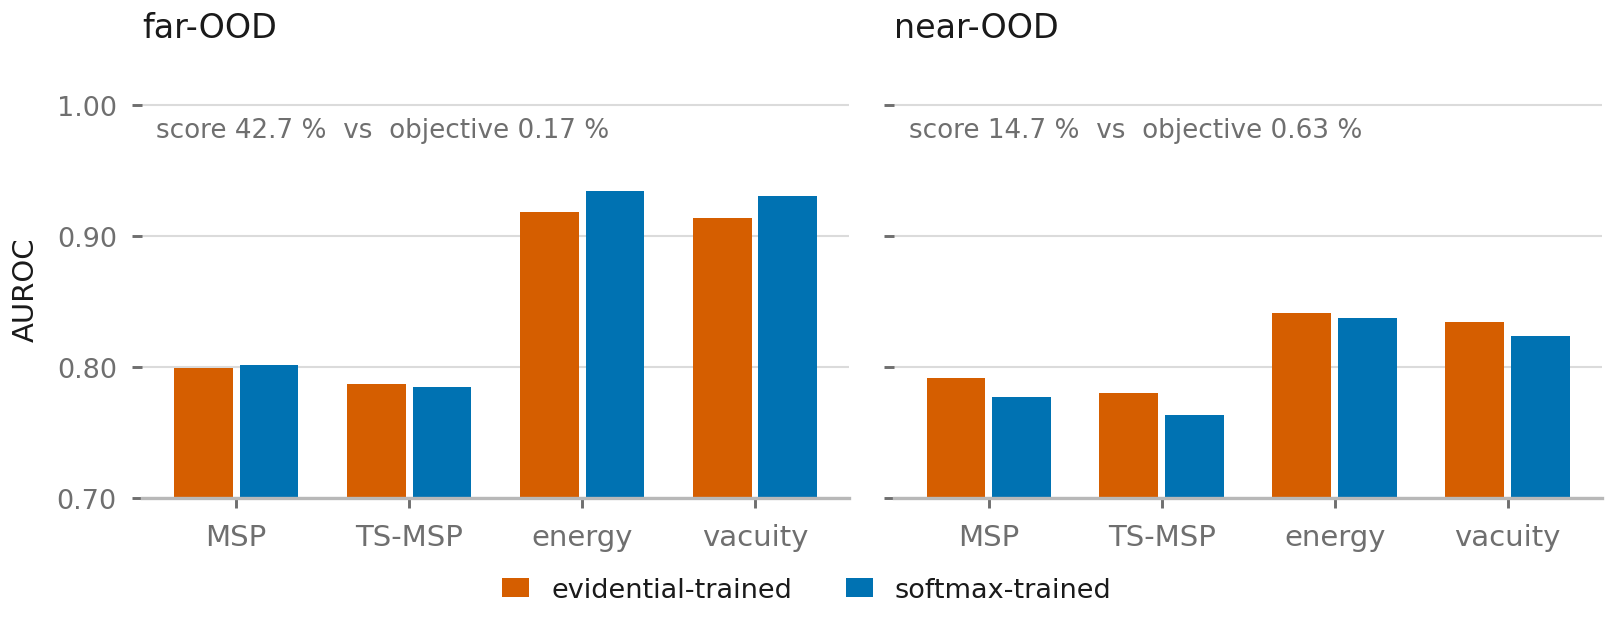
\includegraphics[width=\textwidth]{F12_ood_score_vs_objective.png}
\caption{Mean OOD AUROC by score and by training objective. The same score gives nearly the same AUROC
whichever objective trained the model; the differences between scores are much larger.}
\label{fig:rq2}
\end{figure}

The scoring rule matters far more than the training objective. On far-OOD it explains 42.7\% of the
variance against 0.17\% for the objective; on near-OOD, 14.7\% against 0.63\%. The same score gives almost
the same AUROC whichever objective produced the logits: energy reaches 0.919 on evidential-trained models
and 0.934 on softmax-trained ones, while MSP stays near 0.80 under both. The OOD advantage the evidential
head seemed to offer comes from reading the logits through a score that looks at the absolute strength of
the match (vacuity or energy) rather than at relative class probabilities (MSP), not from evidential
training. This agrees with the theoretical result that softmax is a special case of an evidential
classifier~\cite{hayta2026plugin}. We report the variance shares rather than their ratio: because the
objective's share is close to zero, the ratio is unstable and changed from about $160\times$ to about
$250\times$ when the last 21 models were added to the analysis, while the shares themselves barely
moved.

Related work is close but not identical. Gen{\c{c}} et al.~\cite{genc2026objectives} name the
objective/score confound as an open problem but study no evidential objective, and Krumpl et
al.~\cite{krumpl2026onemodel} cross training methods with detectors at a much larger scale without
evidential models. The part we did not find elsewhere is the cross-application of energy to
Dirichlet-trained logits and the finding that it performs almost the same as on softmax-trained logits.

\section{RQ3: Architecture or Budget?}
\label{sec:rq3}

RQ1 found that the adapter explains only 0.65\% of calibration variance in total. RQ3 asks a different
question: when two adapters are compared directly, which property predicts the winner? A factor can
contribute little total variance and still point in a very consistent direction.

\subsection{Evidence from the grid}

The grid contains 16 matched bottleneck-versus-LoRA pairs (2 datasets $\times$ 2 shot counts $\times$ 2
backbones $\times$ 2 heads), identical except for the adapter.

\begin{table}[H]
\centering
\caption{The 16 matched pairs. Accuracy in \%, gap = bottleneck minus LoRA; better-calibrated adapter in bold.}
\label{tab:pairs}
\small
\begin{adjustbox}{max width=\textwidth}
\begin{tabular}{@{}lllrrrrr@{}}
\toprule
Dataset & Shots & Backbone / head & Acc.\ btl & Acc.\ LoRA & Gap & ECE btl & ECE LoRA \\
\midrule
CIFAR-FS & 1 & ResNet-18 / softmax & 78.57 & 75.44 & $+3.12$ & \textbf{0.056} & 0.097 \\
CIFAR-FS & 1 & ResNet-18 / evid. & 79.19 & 73.76 & $+5.43$ & \textbf{0.277} & 0.297 \\
CIFAR-FS & 5 & ResNet-18 / softmax & 91.44 & 86.25 & $+5.19$ & \textbf{0.067} & 0.102 \\
CIFAR-FS & 5 & ResNet-18 / evid. & 91.58 & 83.33 & $+8.26$ & \textbf{0.301} & 0.329 \\
MiniImageNet & 1 & ResNet-18 / softmax & 85.03 & 80.29 & $+4.75$ & \textbf{0.101} & 0.175 \\
MiniImageNet & 1 & ResNet-18 / evid. & 84.81 & 79.16 & $+5.65$ & \textbf{0.307} & 0.371 \\
MiniImageNet & 5 & ResNet-18 / softmax & 95.56 & 91.56 & $+4.00$ & \textbf{0.085} & 0.193 \\
MiniImageNet & 5 & ResNet-18 / evid. & 95.88 & 88.32 & $+7.56$ & \textbf{0.294} & 0.405 \\
\midrule
CIFAR-FS & 1 & MNv3-S / softmax & 78.80 & 75.43 & $+3.37$ & 0.050 & \textbf{0.029} \\
CIFAR-FS & 1 & MNv3-S / evid. & 78.88 & 74.03 & $+4.85$ & 0.254 & \textbf{0.216} \\
CIFAR-FS & 5 & MNv3-S / softmax & 90.74 & 88.05 & $+2.70$ & 0.070 & \textbf{0.062} \\
CIFAR-FS & 5 & MNv3-S / evid. & 90.24 & 87.52 & $+2.72$ & 0.304 & \textbf{0.293} \\
MiniImageNet & 1 & MNv3-S / softmax & 74.92 & 72.45 & $+2.47$ & 0.065 & \textbf{0.024} \\
MiniImageNet & 1 & MNv3-S / evid. & 75.61 & 72.48 & $+3.14$ & 0.253 & \textbf{0.219} \\
MiniImageNet & 5 & MNv3-S / softmax & 90.10 & 87.96 & $+2.13$ & 0.111 & \textbf{0.096} \\
MiniImageNet & 5 & MNv3-S / evid. & 90.64 & 87.96 & $+2.68$ & 0.318 & \textbf{0.305} \\
\bottomrule
\end{tabular}
\end{adjustbox}
\end{table}

\begin{figure}[H]
\centering
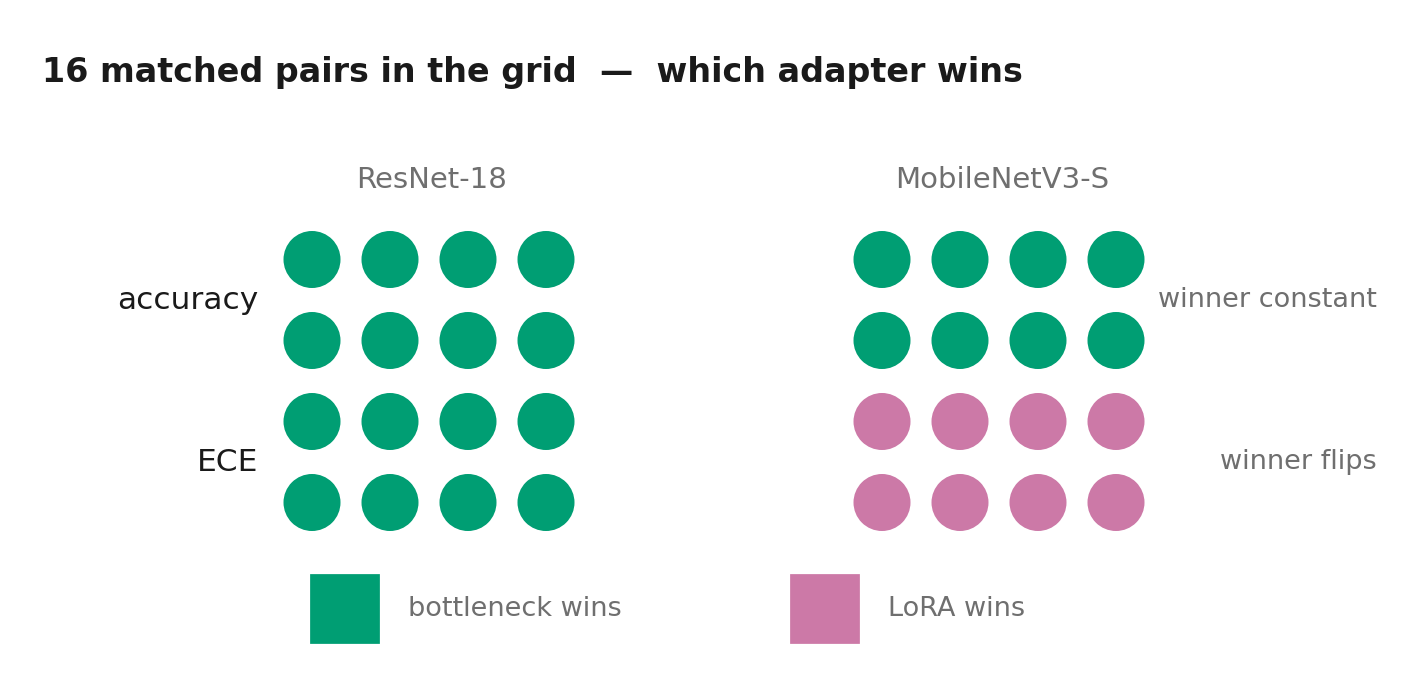
\includegraphics[width=0.75\textwidth]{F13_matched_pairs_deltas.png}
\caption{Which adapter wins each of the 16 pairs. The accuracy winner never changes; the calibration winner
changes with the backbone.}
\label{fig:pairs}
\end{figure}

Two facts stand out (\cref{tab:pairs,fig:pairs}).
\begin{enumerate}
\item \textbf{The accuracy winner does not change when the size ordering reverses.} The bottleneck adapter
is more accurate in all 16 pairs, by 2.1 to 8.3 percentage points, both on ResNet-18, where it has
$2.58\times$ more parameters than LoRA, and on MobileNetV3-Small, where it has $1.55\times$ fewer. Size
cannot explain this, so accuracy follows architecture. The bottleneck also gives the better near-OOD
AUROC in all 16 pairs. For far-OOD (SVHN) it wins only 11 of 16, so we make no claim there.
\item \textbf{The calibration winner flips with the backbone.} The bottleneck is better calibrated in all 8
ResNet-18 pairs and LoRA in all 8 MobileNetV3-Small pairs. The direction is very consistent (a 16-of-16
sign pattern has $p \approx 3 \times 10^{-5}$ under random directions), although the size of the
calibration gap exceeds twice the seed-to-seed spread in only 10 of the 16 pairs, all 8 MiniImageNet
pairs but only 2 of the 8 CIFAR-FS pairs.
\end{enumerate}

The second fact admits two explanations. The better-calibrated adapter is always the \emph{larger} one,
which suggests that calibration follows the parameter budget. But it is also always ``whichever adapter
suits this backbone'', because in this grid the size ordering flips exactly when the backbone changes.
The two explanations predict identical patterns here, so the grid cannot decide between them.

\subsection{The matched-budget experiment}

The pre-registered matched-budget experiment (\cref{sec:matched-design}) removes the size difference
within each backbone. If budget caused the calibration gap, the gap should collapse once the budgets are
equal. \Cref{tab:matched} gives the result for each cell, averaged over the two budget levels, and
\cref{fig:matched} compares it with the grid.

\begin{table}[H]
\centering
\caption{Matched-budget calibration results. $\Delta$ = LoRA ECE minus bottleneck ECE. Collapse ratio =
matched $|\Delta|$ divided by unmatched $|\Delta|$. Per-level numbers are in \cref{tab:matched-levels}.}
\label{tab:matched}
\small
\begin{adjustbox}{max width=\textwidth}
\begin{tabular}{@{}llrrrrrrl@{}}
\toprule
Backbone & Head & ECE btl & ECE LoRA & $\Delta$ matched & $\Delta$ grid & Ratio & $2\sigma$ & Rule fired \\
\midrule
ResNet-18 & evidential & 0.296 & 0.408 & $+0.112$ & $+0.111$ & 1.01 & 0.035 & backbone \\
ResNet-18 & softmax & 0.084 & 0.183 & $+0.099$ & $+0.108$ & 0.92 & 0.012 & backbone \\
MNv3-S & evidential & 0.317 & 0.311 & $-0.006$ & $-0.012$ & 0.50 & 0.002 & backbone \\
MNv3-S & softmax & 0.112 & 0.106 & $-0.006$ & $-0.015$ & 0.61 & 0.015 & none \\
\bottomrule
\end{tabular}
\end{adjustbox}
\end{table}

\begin{figure}[H]
\centering
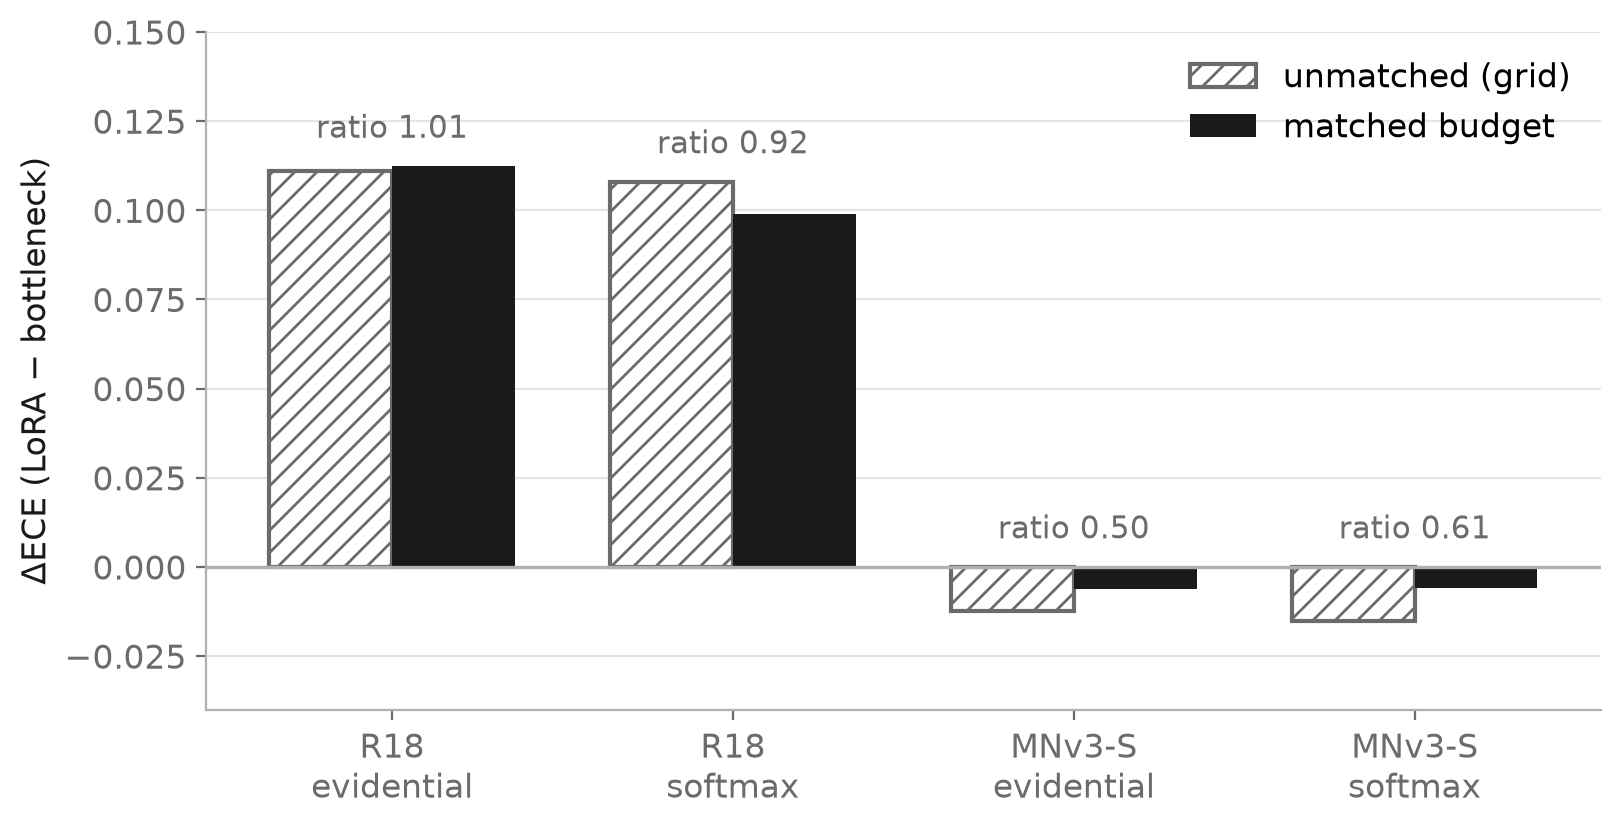
\includegraphics[width=0.85\textwidth]{F14a_matched_budget_bars.png}
\caption{$\Delta$ECE (LoRA $-$ bottleneck) in the grid (hatched) and at matched budget (solid). The labels
give the pre-registered collapse ratios. On ResNet-18 the gap is unchanged; on MobileNetV3-Small it
shrinks but keeps its sign.}
\label{fig:matched}
\end{figure}

\paragraph{Verdict.} The budget rule fired in 0 of 4 cells and the backbone rule in 3 of 4, against a
pre-set threshold of 3; the architecture rule fired in none, because the sign still differs between
backbones. The pre-registered verdict is therefore \emph{backbone}:
\begin{itemize}
\item On ResNet-18, equalising the budgets left the calibration gap where it was (collapse ratios 1.01 and
0.92). At the high budget, for example, the softmax bottleneck has ECE 0.085 and the softmax LoRA 0.173
with almost the same number of parameters. A gap caused by the budget difference should have
disappeared with it.
\item On MobileNetV3-Small, the gap roughly halved (ratios 0.50 and 0.61) but kept its sign. Budget
therefore affects the size of the gap there, but not its direction.
\item The softmax MobileNetV3-Small cell fired no rule: its matched gap ($-0.006$) is smaller than its
noise ($2\sigma = 0.015$), and its two budget levels even disagree in sign.
\item The two backbones are far from symmetric. The ResNet-18 gap (about 0.10) is roughly fifteen times the
MobileNetV3-Small gap (about 0.006), so most of the evidence comes from ResNet-18.
\end{itemize}

\paragraph{The architecture half survives.} At matched budget the bottleneck is still more accurate in
all 8 comparisons and still gives the better near-OOD AUROC in all 8, every time by more than $2\sigma$.
Its accuracy lead ranges from 1.4 points (MobileNetV3-Small, softmax, low budget) to 8.6 points
(ResNet-18, evidential, high budget), and none of the accuracy gaps collapsed (ratios 0.68--1.22). Even
LoRA at rank 41, with the same 31.5K parameters as the bottleneck on ResNet-18, stays 5.8 to 8.6 points
behind. Far-OOD again shows no clear pattern (bottleneck wins 5 of 8).

\paragraph{Answer to RQ3.} Accuracy and near-OOD detection follow adapter architecture, whichever adapter
has more parameters. Calibration follows neither architecture nor budget cleanly: the better-calibrated
adapter depends on the backbone. The reading suggested by the grid alone, that calibration follows the
parameter budget, is not supported. The base-grid interaction analysis points the same way: backbone
$\times$ adapter is the largest two-way interaction for ECE and negligible for accuracy and OOD detection
(\cref{sec:rq1}).

Two caveats apply. ``Architecture'' here means each adapter as implemented: the bottleneck differs from
LoRA in its non-linearity, its placement in four stages instead of one layer, and in adding a branch
instead of changing a weight, and we do not separate these. And with only two backbones we cannot say
which property of the backbone is responsible; depth, width, normalisation, the inverted-residual block
and the scale of the features at the adapter sites all differ between them.

We found no prior work that separates adapter architecture from parameter budget by outcome. The usual
practice in PEFT studies is to compare adapters at equal budgets; Wang et al.~\cite{wang2026cptensor}
study the accuracy-versus-budget curve at a finer resolution but measure accuracy only.

\section{RQ4: Repairing Evidential Calibration}
\label{sec:rq4}

For each of the 60 evidential models we refitted only the scale $a$ and bias $b$ on the validation
episodes, keeping everything else fixed (\cref{sec:refit}).

\begin{figure}[H]
\centering
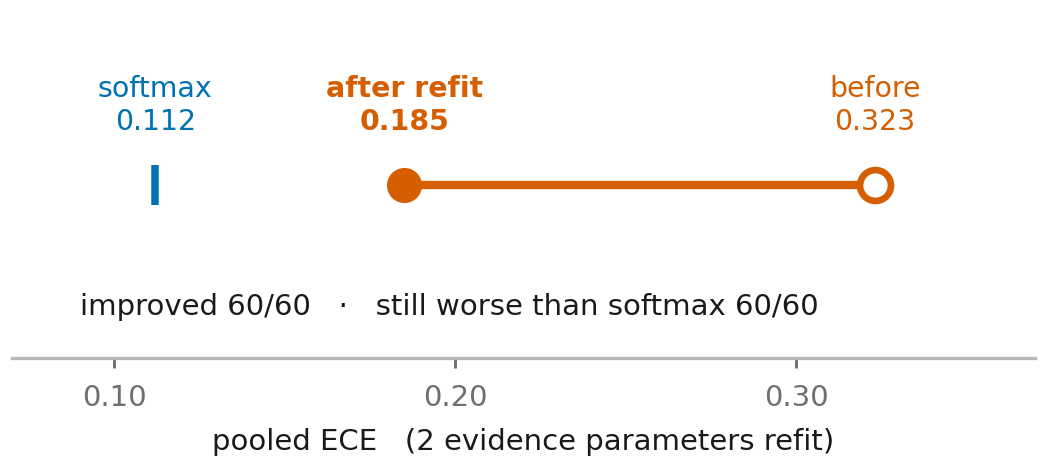
\includegraphics[width=0.8\textwidth]{F15a_ece_before_after_dumbbell.png}
\caption{Mean pooled ECE of the 60 evidential models before and after the refit, against plain softmax
applied to the same logits.}
\label{fig:refit-ece}
\end{figure}

\paragraph{Calibration improves in every model.} The refit lowers pooled ECE in 60 of 60 models, from a
mean of 0.323 to 0.185, with improvements between 0.10 and 0.18 per model. The refitted scale is much
larger than the one learned in training: 3.6 to 14.5 (median 9.0) against 1.5 to 4.5 (median 2.9), with
the bias moving from $-9.3 \ldots -5.6$ to $-26.5 \ldots -8.1$. A larger scale makes evidence grow faster
once a similarity passes the threshold, which sharpens the predictions; this is consistent with the
underconfidence seen in the reliability diagrams. Training the two parameters jointly with the adapter,
under the evidential loss, simply leaves them far from the point that minimises the validation NLL.
Accuracy is essentially unchanged (it moves by at most 0.04 percentage points in any model), as expected
from a refit that keeps the scale positive and so preserves the order of the logits.

\paragraph{It narrows the gap but does not close it.} Even after the refit, the evidential readout is
worse calibrated than a plain softmax over the \emph{same} logits in 60 of 60 models (mean ECE 0.185
against 0.112, on average $2.2\times$ higher, between $1.07\times$ and $5.8\times$), and far worse than the
temperature-scaled softmax (mean ECE 0.023, on average $13.6\times$ higher). A possible reason, which we did
not test, is that bounded cosine logits together with the ``$+1$'' prior on every class limit how much of
the Dirichlet mass the top class can hold.

\paragraph{OOD ranking mostly survives.} Comparing vacuity AUROC before and after the refit for 60 models
and four OOD sets gives 240 comparisons (\cref{fig:refit-ood}). In 192 of them (80\%) the AUROC did not
drop by more than 0.005: it stayed within $\pm 0.005$ in 154 and improved by more than 0.005 in 38. In the
remaining 48 it dropped by more than 0.005, at worst by 0.032 (Gaussian noise, CIFAR-FS 1-shot,
MobileNetV3-Small with LoRA). The mean change is $+0.003$. Reordering does happen, as anticipated in
\cref{sec:refit}: in the worst case the Spearman correlation between the vacuity rankings before and after
the refit is 0.87.

\begin{figure}[H]
\centering
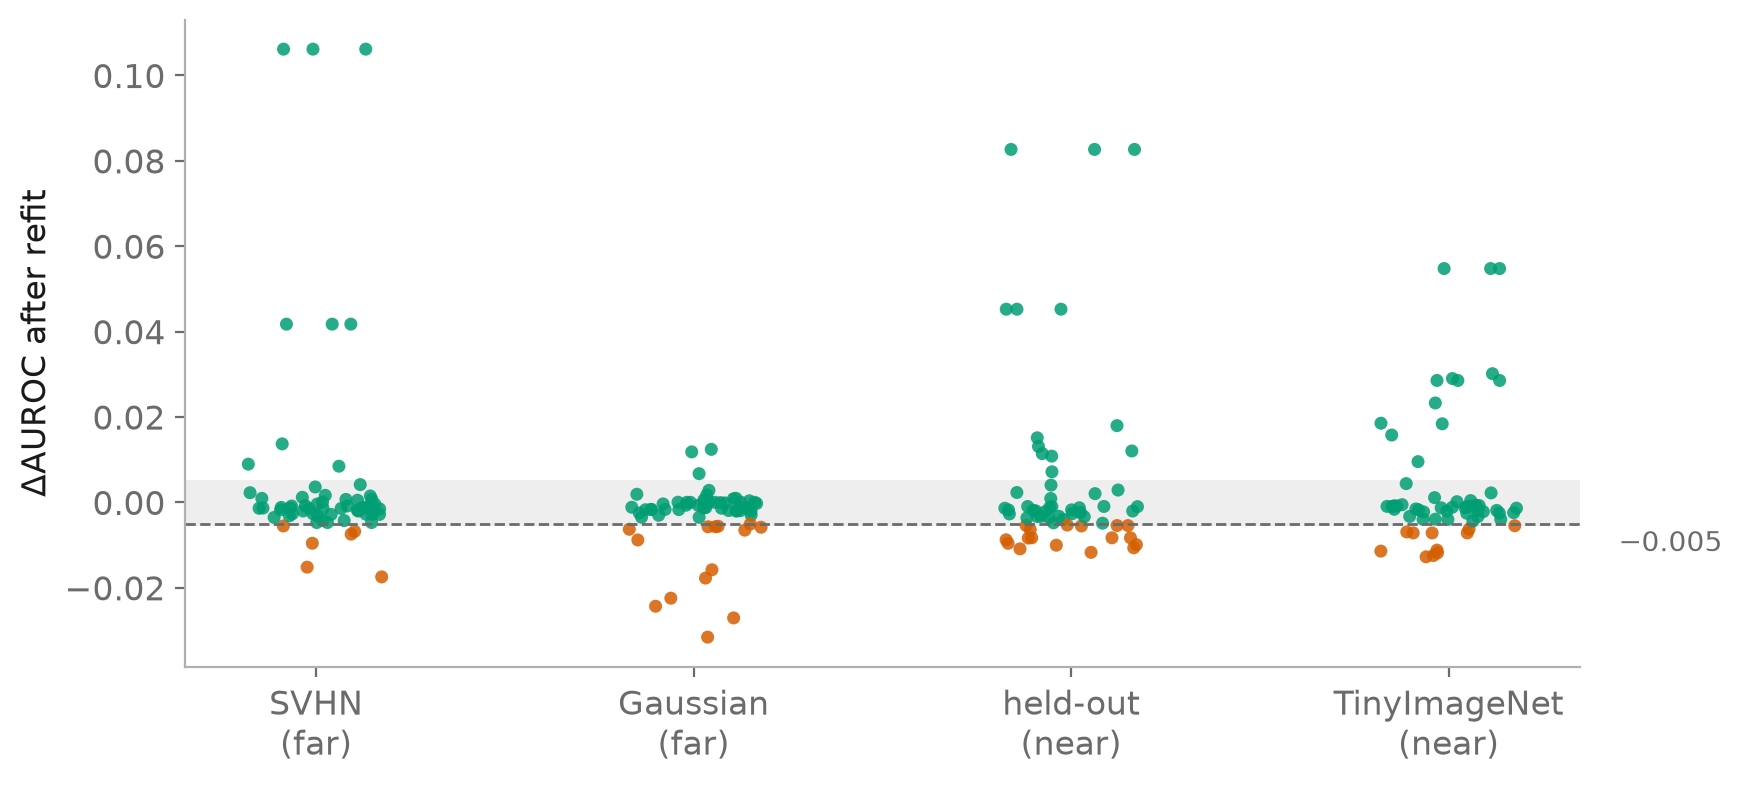
\includegraphics[width=0.85\textwidth]{F15b_delta_auroc_strip.png}
\caption{Change in vacuity AUROC after the refit for each model and OOD set (240 points). Green: did not
drop by more than 0.005. Orange: dropped by more than 0.005.}
\label{fig:refit-ood}
\end{figure}

\paragraph{Answer to RQ4.} The evidential head's calibration can be improved cheaply and reliably after
training, but not repaired: it remains worse calibrated than softmax in every model, and the refit costs a
small but real amount of OOD ranking in a fifth of the comparisons. Post-hoc calibration itself is a mature
field~\cite{guo2017calibration,kull2019dirichlet,zhao2026invlt}, and the size of the improvement is in line
with what temperature scaling and BEL report~\cite{guo2017calibration,linghu2022bel}. What we add is the
measurement of this particular two-parameter refit for an evidential prototype head, including its effect
on the OOD ranking, which existing evidential recalibration methods address by changing the model or its
training instead~\cite{carlotti2026dipedl,turacan2026invascal}.

\section{Deployment Cost}
\label{sec:deployment}

We measured inference latency for the twelve backbone, adapter and head combinations in the grid on a
single CPU thread (\cref{tab:latency,fig:latency}). The backbone dominates: with the
same adapter and head, ResNet-18 takes 62.2 ms per image and MobileNetV3-Small 12.1 ms, a $5.1\times$
difference. Switching the adapter changes latency by only 3.9\% on ResNet-18, and on MobileNetV3-Small LoRA
is 5.8\% faster than the bottleneck even though it has more parameters. The head costs nothing measurable:
the mean latency difference between evidential and softmax heads is 1.3\%, below the 5.9\% run-to-run
noise of the measurement session, and the whole uncertainty computation for a 75-query episode costs about
1\% of one image's forward pass.

\begin{table}[H]
\centering
\caption{Effect of each design choice on CPU inference latency.}
\label{tab:latency}
\begin{adjustbox}{max width=\textwidth}
\begin{tabular}{@{}lr@{}}
\toprule
Design choice & Effect on latency \\
\midrule
Backbone (ResNet-18 vs.\ MobileNetV3-Small) & $5.1\times$ \\
Adapter type & 4--6\% \\
Evidential vs.\ softmax head & about 1\%, within measurement noise \\
\bottomrule
\end{tabular}
\end{adjustbox}
\end{table}

\begin{figure}[H]
\centering
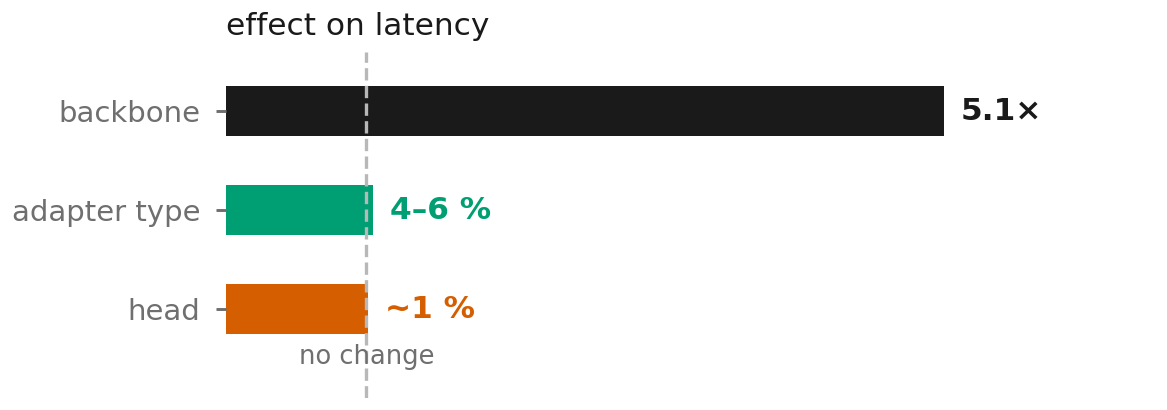
\includegraphics[width=0.75\textwidth]{D3_latency_effect_bars.png}
\caption{Effect of backbone, adapter type and head on single-thread CPU latency.}
\label{fig:latency}
\end{figure}

Put together with the earlier sections, this gives a simple division of labour. The backbone decides the
latency; the adapter decides most of the accuracy that the shot count leaves open; the head decides
calibration but costs nothing at inference. Given RQ2 and RQ4, a softmax head with temperature scaling for
confidence and the energy score for OOD detection is the stronger default in our grid; the evidential head
is worth choosing only if a bounded ``I don't know'' score such as vacuity is specifically needed.

\section{Comparison with Published Few-Shot Results}
\label{sec:sota}

Our absolute accuracies should be read with care. Our backbones are pretrained on ImageNet, while classic
few-shot methods such as MetaOptNet train from scratch on the 64 base classes, and MiniImageNet's test
classes are themselves ImageNet classes that our backbones saw during pretraining. \Cref{tab:sota}
therefore places our results next to published numbers for orientation, not as a claim of state-of-the-art
accuracy.

\begin{table}[H]
\centering
\caption{Accuracy (\%) on 5-way episodes next to published results. P>M>F rows are from Hu et
al.~\cite{hu2022pmf}; these methods train the whole backbone. Our backbones are frozen.}
\label{tab:sota}
\small
\begin{adjustbox}{max width=\textwidth}
\begin{tabular}{@{}llrrrrr@{}}
\toprule
& & Trainable & \multicolumn{2}{c}{CIFAR-FS} & \multicolumn{2}{c}{MiniImageNet} \\
\cmidrule(lr){4-5}\cmidrule(lr){6-7}
Method & Backbone & params & 1-shot & 5-shot & 1-shot & 5-shot \\
\midrule
P>M>F, Sup-21k $\rightarrow$ ProtoNet & ViT-B/16 & $\sim$86M & 92.3 & 96.7 & 97.2 & 99.2 \\
P>M>F, DINO $\rightarrow$ ProtoNet & ViT-B/16 & $\sim$86M & 84.3 & 92.2 & 95.3 & 98.4 \\
P>M>F, DINO $\rightarrow$ ProtoNet & ViT-S/16 & $\sim$21M & 81.1 & 92.5 & 93.1 & 98.0 \\
P>M>F, DINO $\rightarrow$ ProtoNet & ResNet-50 & $\sim$25M & -- & -- & 79.2 & 92.0 \\
BEL$^{\dagger}$~\cite{linghu2022bel} & ResNet-12 & full & 73.96 & 86.92 & 63.10 & 79.60 \\
MetaOptNet-SVM~\cite{lee2019metaoptnet} & ResNet-12 & full & 72.0 & 84.2 & 62.64 & 78.63 \\
\midrule
Ours, bottleneck, softmax & ResNet-18 & 31,744 & 78.57 & 91.44 & 85.03 & 95.56 \\
Ours, bottleneck, softmax & MobileNetV3-S & 6,928 & 78.80 & 90.74 & 74.92 & 90.10 \\
\bottomrule
\multicolumn{7}{@{}l}{\footnotesize $^{\dagger}$ CIFAR-FS numbers are for DeepEMD+BEL and MiniImageNet numbers for Meta-Baseline+BEL.}
\end{tabular}
\end{adjustbox}
\end{table}

On CIFAR-FS 5-shot, the frozen ResNet-18 with a 31.7K-parameter adapter is 1.1 points behind DINO
ViT-S/16 trained end to end ($662\times$ more trainable parameters) and 0.8 points behind DINO ViT-B/16.
On MiniImageNet it is ahead of the ResNet-50 P>M>F variant (95.56 against 92.0 at 5-shot), although the
ImageNet overlap favours us there. At 1-shot and with the smaller backbone the gap is large: MobileNetV3-Small
reaches 74.92\% on MiniImageNet 1-shot against 93.1\% for DINO ViT-S/16. None of the methods in the table
reports calibration or OOD detection.

\section{Limitations}
\label{sec:limits}

\begin{enumerate}
\item \textbf{ImageNet pretraining overlap.} Both backbones were pretrained on ImageNet, which contains
MiniImageNet's test classes. Absolute accuracies are not comparable with from-scratch few-shot results.
Our research questions concern differences between design choices under the same backbones, which limits
but does not remove the effect.
\item \textbf{Two backbones.} We can show that calibration depends on the backbone but not why. Answering
that needs more backbones that vary one property at a time.
\item \textbf{One shared recipe.} All configurations use one training recipe, chosen once and not tuned per
configuration. The study answers how the factors compare under that recipe, not what the best achievable
number for each configuration is.
\item \textbf{Three seeds, varying initialisation only.} The seed changes the adapter's initialisation but
not the training episodes, so seed-to-seed spread understates the full training variability. The two
baselines have no seed variation at all. Small differences should be read with caution.
\item \textbf{Near-OOD overlap with validation classes.} The held-out near-OOD pools come from the
validation classes that were also used for model selection and fitting. TinyImageNet does not have this
overlap, which is why RQ1 uses it.
\item \textbf{No data augmentation and a cosine head only.} Both were held fixed across all
configurations, so they affect absolute numbers more than comparisons, but we did not measure their
effect.
\item \textbf{Literature coverage.} Our statements that we found no prior work on a point rest on a
careful but necessarily incomplete search.
\end{enumerate}

\chapter{Conclusion}
\label{ch:conclusion}

\section{Summary of Findings}

We set out to learn which design choices govern which aspects of reliability when a frozen lightweight
CNN is adapted for few-shot classification with a small trainable adapter. \Cref{tab:conclusion}
summarises the answers.

\begin{table}[H]
\centering
\caption{What this thesis found: no single design choice optimises every reliability aspect.}
\label{tab:conclusion}
\begin{tabularx}{\textwidth}{@{}l>{\raggedright\arraybackslash}p{3.6cm}X@{}}
\toprule
Aspect & Main factor & Evidence \\
\midrule
Accuracy & shot count, then adapter architecture & 76\% of accuracy variance from shots; bottleneck wins 16/16 grid pairs and 8/8 at matched budget \\
Calibration & head, then backbone & 83\% of ECE variance from the head; at matched budget, backbone rule 3/4 cells, budget rule 0/4 \\
OOD detection & scoring rule & 42.7\% of far-OOD variance from the score vs.\ 0.17\% from the training objective \\
Calibration repair & two-parameter refit & ECE improved in 60/60 evidential models, still worse than softmax in 60/60 \\
\bottomrule
\end{tabularx}
\end{table}

A 31.7K-parameter parallel bottleneck adapter beats full fine-tuning of an 11.18M-parameter ResNet-18 at
5-shot and comes within 2.6 points of it at 1-shot. Accuracy is driven mainly by the number
of shots and then by the adapter's architecture, and the head barely affects it. Calibration is driven by
the head: the evidential head is worse calibrated than softmax in all 20 matched pairs. The evidential head
looked like a better OOD detector, but separating training objective from scoring rule shows that this
advantage belongs to the score; the parameter-free energy score is the strongest score in most settings and
works almost equally well on evidential-trained logits. When the two adapters are given the same parameter
budget, the bottleneck still wins on accuracy and near-OOD detection, while the calibration gap stays with
the backbone. Finally, refitting the evidential head's two evidence parameters after training improves its
calibration in every model but does not make it as well calibrated as softmax, and it lowers OOD AUROC by more
than 0.005 in a fifth of the comparisons.

\begin{figure}[H]
\centering
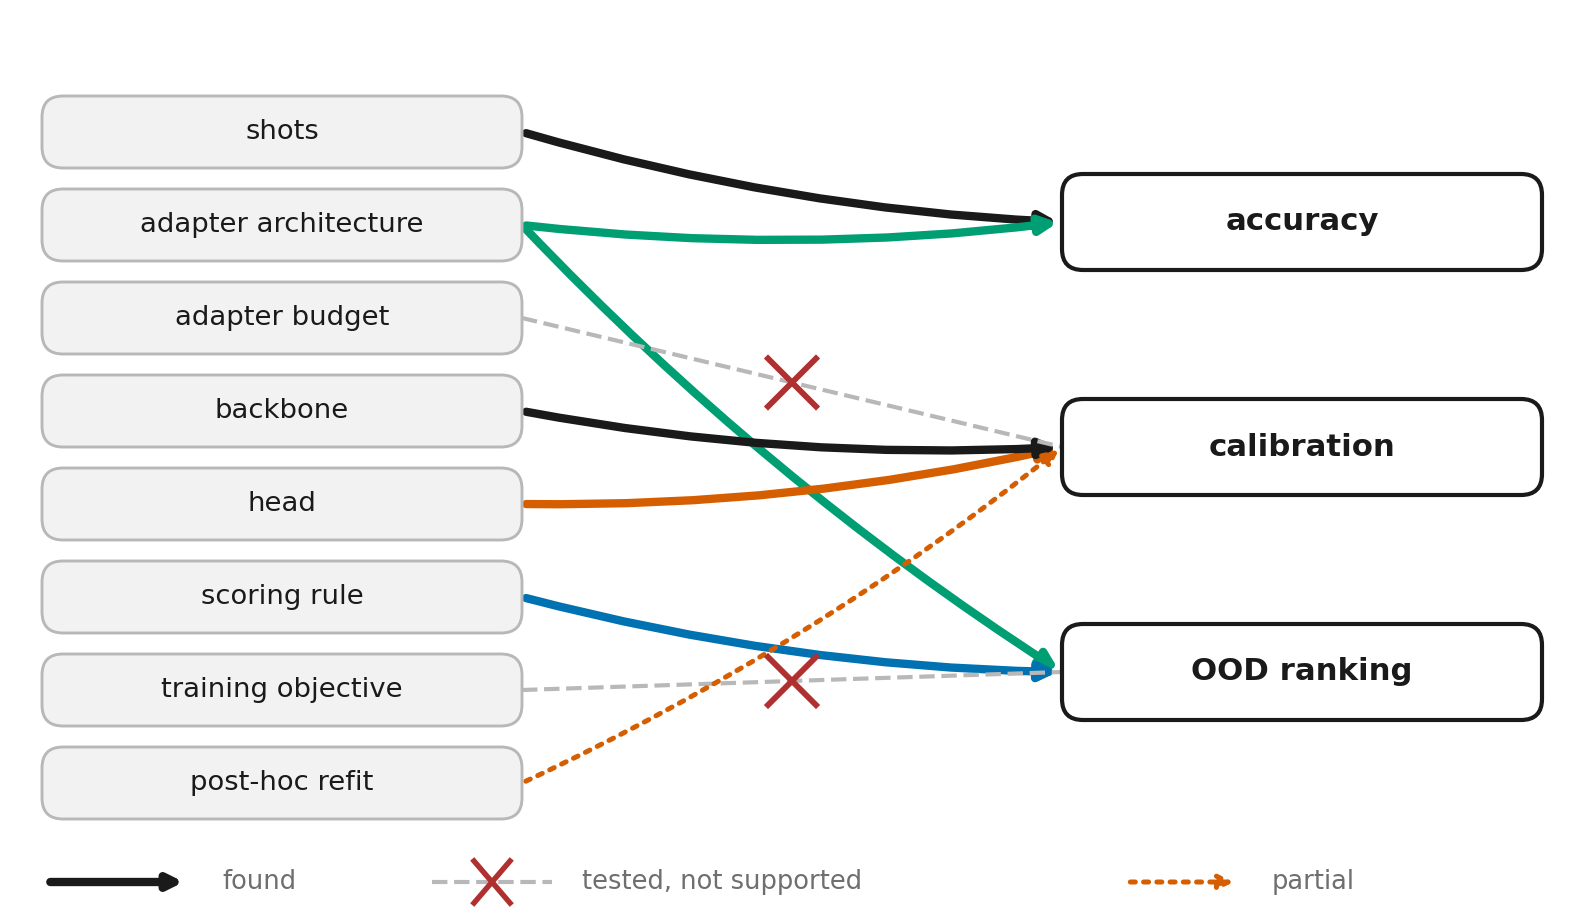
\includegraphics[width=0.9\textwidth]{F16_findings_graph.png}
\caption{Each design factor against each reliability outcome: links that were found, links that were tested
and not supported, and partial links.}
\label{fig:findings}
\end{figure}

The main contribution is therefore not a better model but a controlled decomposition of which design
choices govern which aspects of reliability in this few-shot PEFT setting.

\section{Contributions}

\begin{itemize}
\item A controlled comparison of adapters on frozen lightweight CNNs that reports accuracy, calibration and
OOD detection for the same 120 models.
\item A variance decomposition showing that accuracy and calibration are controlled by largely different
factors (RQ1).
\item A crossing of training objectives with scoring rules showing that OOD detection is decided by the
score, including the finding that energy transfers almost unchanged to evidential-trained models (RQ2).
\item A pre-registered matched-budget design that separates adapter architecture from parameter budget and
shows that calibration follows the backbone, not the budget (RQ3).
\item A measured two-parameter post-hoc refit of the evidential head, reporting both its benefit and its
cost in OOD ranking (RQ4).
\end{itemize}

\section{Limitations}

The limitations are discussed in \cref{sec:limits}. The most important are the ImageNet pretraining
overlap with MiniImageNet's test classes, the use of only two backbones, a single shared training recipe,
and three seeds that vary only the adapter's initialisation.

\section{Future Work}

\begin{itemize}
\item \textbf{More backbones.} The most important next step is to add backbones that vary depth, width,
normalisation and block type one at a time, to find which backbone property decides which adapter is better
calibrated.
\item \textbf{Separating the parts of ``architecture''.} Variants of the two adapters that differ in only one
respect (non-linearity, number of insertion points, or branch versus weight update) would show what makes
the bottleneck more accurate.
\item \textbf{A transformer arm.} Running a small ViT under exactly our protocol would replace the
literature comparison of \cref{sec:sota} with a direct measurement.
\item \textbf{Pretraining control.} A backbone pretrained without the MiniImageNet test classes would measure
the size of the pretraining overlap instead of only noting it.
\end{itemize}

\section{Concluding Remarks}

We began by asking whether an evidential uncertainty mechanism makes a parameter-efficient, lightweight CNN
more reliable in the few-shot regime. The answer turned out to be more specific than yes or no. The
evidential head ranks unfamiliar inputs better than softmax probabilities do, but a free score on ordinary
softmax logits does as well or better in most settings, and the evidential head pays for it with worse calibration that a
small post-hoc refit only partly repairs. Which adapter to use, which backbone to use and how to score
uncertainty each turned out to matter for a different part of reliability, and only a controlled design
could tell them apart.


\clearpage
\phantomsection
\addcontentsline{toc}{chapter}{References}
\renewcommand{\bibname}{References}
\bibliographystyle{IEEEtran}
\bibliography{refs}

\appendix
\chapter{Full Result Tables}
\label{app:tables}

All values are means over three training seeds (42, 43, 44), each evaluated on the same 600 test
episodes. MNv3-S stands for MobileNetV3-Small and MiniIN for MiniImageNet. Rows marked $^\ast$ are the baselines (ResNet-18, CIFAR-FS only). The CIFAR-FS 5-shot
MobileNetV3-Small LoRA evidential row uses the corrected seed-42 run described at the start of
\cref{ch:results}.


\begingroup\footnotesize\setlength{\tabcolsep}{3.5pt}
\begin{longtable}{@{}lllllrrr@{}}
\caption{Accuracy, macro-F1 and trainable parameters for all 40 configurations.}\label{tab:app-acc}\\
\toprule
Dataset & Shots & Backbone & Adapter & Head & Params & Acc.\ (\%) & Macro-F1 (\%)\\
\midrule
\endfirsthead
\multicolumn{8}{@{}l}{\emph{\cref{tab:app-acc}, continued}}\\
\toprule
Dataset & Shots & Backbone & Adapter & Head & Params & Acc.\ (\%) & Macro-F1 (\%)\\
\midrule
\endhead
\bottomrule
\endfoot
CIFAR-FS & 1 & ResNet-18 & Bottleneck & Evid. & 31,746 & 79.19 & 78.29 \\
 &  &  & Bottleneck & Softmax & 31,744 & 78.57 & 77.50 \\
 &  &  & LoRA & Evid. & 12,290 & 73.76 & 72.61 \\
 &  &  & LoRA & Softmax & 12,288 & 75.44 & 74.33 \\
 &  &  & Full FT$^\ast$ & Evid. & 11,176,514 & 80.36 & 79.14 \\
 &  &  & Full FT$^\ast$ & Softmax & 11,176,512 & 81.14 & 80.02 \\
 &  &  & Lin.\ probe$^\ast$ & Evid. & 2 & 70.25 & 69.10 \\
 &  &  & Lin.\ probe$^\ast$ & Softmax & 0 & 70.25 & 69.10 \\
 &  & MNv3-S & Bottleneck & Evid. & 6,930 & 78.88 & 77.83 \\
 &  &  & Bottleneck & Softmax & 6,928 & 78.80 & 77.69 \\
 &  &  & LoRA & Evid. & 10,754 & 74.03 & 72.47 \\
 &  &  & LoRA & Softmax & 10,752 & 75.43 & 74.09 \\
 & 5 & ResNet-18 & Bottleneck & Evid. & 31,746 & 91.58 & 91.46 \\
 &  &  & Bottleneck & Softmax & 31,744 & 91.44 & 91.29 \\
 &  &  & LoRA & Evid. & 12,290 & 83.33 & 82.96 \\
 &  &  & LoRA & Softmax & 12,288 & 86.25 & 85.98 \\
 &  &  & Full FT$^\ast$ & Evid. & 11,176,514 & 88.82 & 88.56 \\
 &  &  & Full FT$^\ast$ & Softmax & 11,176,512 & 90.47 & 90.27 \\
 &  &  & Lin.\ probe$^\ast$ & Evid. & 2 & 87.41 & 87.28 \\
 &  &  & Lin.\ probe$^\ast$ & Softmax & 0 & 87.41 & 87.28 \\
 &  & MNv3-S & Bottleneck & Evid. & 6,930 & 90.24 & 90.08 \\
 &  &  & Bottleneck & Softmax & 6,928 & 90.74 & 90.59 \\
 &  &  & LoRA & Evid. & 10,754 & 87.52 & 87.25 \\
 &  &  & LoRA & Softmax & 10,752 & 88.05 & 87.79 \\
MiniIN & 1 & ResNet-18 & Bottleneck & Evid. & 31,746 & 84.81 & 84.21 \\
 &  &  & Bottleneck & Softmax & 31,744 & 85.03 & 84.34 \\
 &  &  & LoRA & Evid. & 12,290 & 79.16 & 78.11 \\
 &  &  & LoRA & Softmax & 12,288 & 80.29 & 79.36 \\
 &  & MNv3-S & Bottleneck & Evid. & 6,930 & 75.61 & 74.53 \\
 &  &  & Bottleneck & Softmax & 6,928 & 74.92 & 73.71 \\
 &  &  & LoRA & Evid. & 10,754 & 72.48 & 70.97 \\
 &  &  & LoRA & Softmax & 10,752 & 72.45 & 70.98 \\
 & 5 & ResNet-18 & Bottleneck & Evid. & 31,746 & 95.88 & 95.85 \\
 &  &  & Bottleneck & Softmax & 31,744 & 95.56 & 95.53 \\
 &  &  & LoRA & Evid. & 12,290 & 88.32 & 88.20 \\
 &  &  & LoRA & Softmax & 12,288 & 91.56 & 91.48 \\
 &  & MNv3-S & Bottleneck & Evid. & 6,930 & 90.64 & 90.55 \\
 &  &  & Bottleneck & Softmax & 6,928 & 90.10 & 89.97 \\
 &  &  & LoRA & Evid. & 10,754 & 87.96 & 87.79 \\
 &  &  & LoRA & Softmax & 10,752 & 87.96 & 87.82 \\
\end{longtable}
\endgroup


\begingroup\footnotesize\setlength{\tabcolsep}{3.5pt}
\begin{longtable}{@{}lllllrrrr@{}}
\caption{Calibration: pooled ECE, per-episode ECE, Brier score, and pooled ECE after temperature scaling (softmax heads only).}\label{tab:app-cal}\\
\toprule
Dataset & Shots & Backbone & Adapter & Head & ECE & ECE/ep. & Brier & ECE (TS)\\
\midrule
\endfirsthead
\multicolumn{9}{@{}l}{\emph{\cref{tab:app-cal}, continued}}\\
\toprule
Dataset & Shots & Backbone & Adapter & Head & ECE & ECE/ep. & Brier & ECE (TS)\\
\midrule
\endhead
\bottomrule
\endfoot
CIFAR-FS & 1 & ResNet-18 & Bottleneck & Evid. & 0.2765 & 0.2885 & 0.4050 & -- \\
 &  &  & Bottleneck & Softmax & 0.0560 & 0.1364 & 0.3084 & 0.0297 \\
 &  &  & LoRA & Evid. & 0.2970 & 0.3096 & 0.4959 & -- \\
 &  &  & LoRA & Softmax & 0.0969 & 0.1592 & 0.3579 & 0.0248 \\
 &  &  & Full FT$^\ast$ & Evid. & 0.3207 & 0.3290 & 0.4254 & -- \\
 &  &  & Full FT$^\ast$ & Softmax & 0.0854 & 0.1468 & 0.2850 & 0.0223 \\
 &  &  & Lin.\ probe$^\ast$ & Evid. & 0.4397 & 0.4397 & 0.7038 & -- \\
 &  &  & Lin.\ probe$^\ast$ & Softmax & 0.2818 & 0.2944 & 0.5283 & 0.0642 \\
 &  & MNv3-S & Bottleneck & Evid. & 0.2540 & 0.2702 & 0.3973 & -- \\
 &  &  & Bottleneck & Softmax & 0.0499 & 0.1347 & 0.3070 & 0.0322 \\
 &  &  & LoRA & Evid. & 0.2156 & 0.2423 & 0.4361 & -- \\
 &  &  & LoRA & Softmax & 0.0287 & 0.1357 & 0.3461 & 0.0403 \\
 & 5 & ResNet-18 & Bottleneck & Evid. & 0.3010 & 0.3070 & 0.2513 & -- \\
 &  &  & Bottleneck & Softmax & 0.0670 & 0.0989 & 0.1332 & 0.0152 \\
 &  &  & LoRA & Evid. & 0.3294 & 0.3366 & 0.3888 & -- \\
 &  &  & LoRA & Softmax & 0.1016 & 0.1353 & 0.2156 & 0.0158 \\
 &  &  & Full FT$^\ast$ & Evid. & 0.3383 & 0.3423 & 0.3220 & -- \\
 &  &  & Full FT$^\ast$ & Softmax & 0.0728 & 0.1048 & 0.1536 & 0.0135 \\
 &  &  & Lin.\ probe$^\ast$ & Evid. & 0.6234 & 0.6234 & 0.7078 & -- \\
 &  &  & Lin.\ probe$^\ast$ & Softmax & 0.4476 & 0.4516 & 0.4554 & 0.0297 \\
 &  & MNv3-S & Bottleneck & Evid. & 0.3043 & 0.3117 & 0.2708 & -- \\
 &  &  & Bottleneck & Softmax & 0.0703 & 0.1039 & 0.1464 & 0.0074 \\
 &  &  & LoRA & Evid. & 0.2925 & 0.3023 & 0.2990 & -- \\
 &  &  & LoRA & Softmax & 0.0616 & 0.1065 & 0.1793 & 0.0060 \\
MiniIN & 1 & ResNet-18 & Bottleneck & Evid. & 0.3073 & 0.3158 & 0.3523 & -- \\
 &  &  & Bottleneck & Softmax & 0.1012 & 0.1416 & 0.2352 & 0.0073 \\
 &  &  & LoRA & Evid. & 0.3708 & 0.3785 & 0.4909 & -- \\
 &  &  & LoRA & Softmax & 0.1748 & 0.2035 & 0.3282 & 0.0077 \\
 &  & MNv3-S & Bottleneck & Evid. & 0.2534 & 0.2664 & 0.4402 & -- \\
 &  &  & Bottleneck & Softmax & 0.0650 & 0.1433 & 0.3551 & 0.0063 \\
 &  &  & LoRA & Evid. & 0.2194 & 0.2417 & 0.4557 & -- \\
 &  &  & LoRA & Softmax & 0.0242 & 0.1368 & 0.3796 & 0.0118 \\
 & 5 & ResNet-18 & Bottleneck & Evid. & 0.2938 & 0.2993 & 0.1883 & -- \\
 &  &  & Bottleneck & Softmax & 0.0850 & 0.1014 & 0.0856 & 0.0057 \\
 &  &  & LoRA & Evid. & 0.4049 & 0.4093 & 0.3977 & -- \\
 &  &  & LoRA & Softmax & 0.1930 & 0.2063 & 0.1913 & 0.0187 \\
 &  & MNv3-S & Bottleneck & Evid. & 0.3177 & 0.3229 & 0.2817 & -- \\
 &  &  & Bottleneck & Softmax & 0.1107 & 0.1339 & 0.1699 & 0.0211 \\
 &  &  & LoRA & Evid. & 0.3053 & 0.3119 & 0.3095 & -- \\
 &  &  & LoRA & Softmax & 0.0955 & 0.1276 & 0.1938 & 0.0221 \\
\end{longtable}
\endgroup


\begingroup\footnotesize\setlength{\tabcolsep}{3.5pt}
\begin{longtable}{@{}lllllrrrr@{}}
\caption{OOD AUROC with each head's native score (vacuity for evidential, MSP for softmax). ``Held-out'' is the 16 validation classes of the same dataset.}\label{tab:app-auroc}\\
\toprule
Dataset & Shots & Backbone & Adapter & Head & SVHN & Gauss. & Held-out & TIN\\
\midrule
\endfirsthead
\multicolumn{9}{@{}l}{\emph{\cref{tab:app-auroc}, continued}}\\
\toprule
Dataset & Shots & Backbone & Adapter & Head & SVHN & Gauss. & Held-out & TIN\\
\midrule
\endhead
\bottomrule
\endfoot
CIFAR-FS & 1 & ResNet-18 & Bottleneck & Evid. & 0.876 & 0.948 & 0.794 & 0.831 \\
 &  &  & Bottleneck & Softmax & 0.784 & 0.826 & 0.696 & 0.738 \\
 &  &  & LoRA & Evid. & 0.833 & 0.940 & 0.725 & 0.771 \\
 &  &  & LoRA & Softmax & 0.747 & 0.686 & 0.667 & 0.710 \\
 &  &  & Full FT$^\ast$ & Evid. & 0.880 & 0.990 & 0.791 & 0.831 \\
 &  &  & Full FT$^\ast$ & Softmax & 0.835 & 0.906 & 0.735 & 0.793 \\
 &  &  & Lin.\ probe$^\ast$ & Evid. & 0.682 & 1.000 & 0.580 & 0.868 \\
 &  &  & Lin.\ probe$^\ast$ & Softmax & 0.672 & 0.733 & 0.663 & 0.728 \\
 &  & MNv3-S & Bottleneck & Evid. & 0.832 & 0.955 & 0.800 & 0.870 \\
 &  &  & Bottleneck & Softmax & 0.750 & 0.861 & 0.723 & 0.787 \\
 &  &  & LoRA & Evid. & 0.818 & 0.768 & 0.743 & 0.747 \\
 &  &  & LoRA & Softmax & 0.756 & 0.803 & 0.670 & 0.698 \\
 & 5 & ResNet-18 & Bottleneck & Evid. & 0.917 & 0.981 & 0.903 & 0.926 \\
 &  &  & Bottleneck & Softmax & 0.885 & 0.936 & 0.818 & 0.852 \\
 &  &  & LoRA & Evid. & 0.890 & 0.981 & 0.814 & 0.849 \\
 &  &  & LoRA & Softmax & 0.820 & 0.860 & 0.742 & 0.782 \\
 &  &  & Full FT$^\ast$ & Evid. & 0.909 & 0.995 & 0.868 & 0.897 \\
 &  &  & Full FT$^\ast$ & Softmax & 0.894 & 0.910 & 0.826 & 0.867 \\
 &  &  & Lin.\ probe$^\ast$ & Evid. & 0.708 & 1.000 & 0.584 & 0.886 \\
 &  &  & Lin.\ probe$^\ast$ & Softmax & 0.855 & 0.812 & 0.797 & 0.843 \\
 &  & MNv3-S & Bottleneck & Evid. & 0.944 & 0.962 & 0.879 & 0.919 \\
 &  &  & Bottleneck & Softmax & 0.845 & 0.862 & 0.832 & 0.886 \\
 &  &  & LoRA & Evid. & 0.925 & 0.990 & 0.855 & 0.881 \\
 &  &  & LoRA & Softmax & 0.829 & 0.910 & 0.787 & 0.810 \\
MiniIN & 1 & ResNet-18 & Bottleneck & Evid. & 0.914 & 0.890 & 0.852 & 0.870 \\
 &  &  & Bottleneck & Softmax & 0.816 & 0.758 & 0.789 & 0.810 \\
 &  &  & LoRA & Evid. & 0.960 & 0.962 & 0.780 & 0.774 \\
 &  &  & LoRA & Softmax & 0.809 & 0.697 & 0.740 & 0.774 \\
 &  & MNv3-S & Bottleneck & Evid. & 0.881 & 0.895 & 0.780 & 0.856 \\
 &  &  & Bottleneck & Softmax & 0.733 & 0.755 & 0.714 & 0.743 \\
 &  &  & LoRA & Evid. & 0.832 & 0.865 & 0.757 & 0.790 \\
 &  &  & LoRA & Softmax & 0.638 & 0.600 & 0.668 & 0.689 \\
 & 5 & ResNet-18 & Bottleneck & Evid. & 0.973 & 0.958 & 0.941 & 0.958 \\
 &  &  & Bottleneck & Softmax & 0.911 & 0.861 & 0.897 & 0.912 \\
 &  &  & LoRA & Evid. & 0.984 & 0.983 & 0.850 & 0.869 \\
 &  &  & LoRA & Softmax & 0.918 & 0.717 & 0.822 & 0.849 \\
 &  & MNv3-S & Bottleneck & Evid. & 0.910 & 0.928 & 0.876 & 0.911 \\
 &  &  & Bottleneck & Softmax & 0.795 & 0.775 & 0.820 & 0.844 \\
 &  &  & LoRA & Evid. & 0.912 & 0.913 & 0.848 & 0.890 \\
 &  &  & LoRA & Softmax & 0.751 & 0.747 & 0.766 & 0.792 \\
\end{longtable}
\endgroup


\begingroup\footnotesize\setlength{\tabcolsep}{3.5pt}
\begin{longtable}{@{}lllllrrrr@{}}
\caption{OOD FPR@95\%TPR with each head's native score (lower is better).}\label{tab:app-fpr}\\
\toprule
Dataset & Shots & Backbone & Adapter & Head & SVHN & Gauss. & Held-out & TIN\\
\midrule
\endfirsthead
\multicolumn{9}{@{}l}{\emph{\cref{tab:app-fpr}, continued}}\\
\toprule
Dataset & Shots & Backbone & Adapter & Head & SVHN & Gauss. & Held-out & TIN\\
\midrule
\endhead
\bottomrule
\endfoot
CIFAR-FS & 1 & ResNet-18 & Bottleneck & Evid. & 0.507 & 0.292 & 0.656 & 0.620 \\
 &  &  & Bottleneck & Softmax & 0.742 & 0.686 & 0.839 & 0.799 \\
 &  &  & LoRA & Evid. & 0.623 & 0.322 & 0.731 & 0.677 \\
 &  &  & LoRA & Softmax & 0.770 & 0.864 & 0.854 & 0.817 \\
 &  &  & Full FT$^\ast$ & Evid. & 0.497 & 0.061 & 0.644 & 0.607 \\
 &  &  & Full FT$^\ast$ & Softmax & 0.647 & 0.489 & 0.775 & 0.714 \\
 &  &  & Lin.\ probe$^\ast$ & Evid. & 0.876 & 0.000 & 0.898 & 0.580 \\
 &  &  & Lin.\ probe$^\ast$ & Softmax & 0.887 & 0.775 & 0.889 & 0.827 \\
 &  & MNv3-S & Bottleneck & Evid. & 0.588 & 0.234 & 0.657 & 0.533 \\
 &  &  & Bottleneck & Softmax & 0.761 & 0.581 & 0.806 & 0.732 \\
 &  &  & LoRA & Evid. & 0.649 & 0.625 & 0.742 & 0.744 \\
 &  &  & LoRA & Softmax & 0.772 & 0.724 & 0.849 & 0.825 \\
 & 5 & ResNet-18 & Bottleneck & Evid. & 0.424 & 0.120 & 0.411 & 0.325 \\
 &  &  & Bottleneck & Softmax & 0.533 & 0.379 & 0.660 & 0.599 \\
 &  &  & LoRA & Evid. & 0.473 & 0.117 & 0.599 & 0.526 \\
 &  &  & LoRA & Softmax & 0.638 & 0.622 & 0.748 & 0.706 \\
 &  &  & Full FT$^\ast$ & Evid. & 0.392 & 0.016 & 0.488 & 0.437 \\
 &  &  & Full FT$^\ast$ & Softmax & 0.434 & 0.478 & 0.605 & 0.534 \\
 &  &  & Lin.\ probe$^\ast$ & Evid. & 0.866 & 0.000 & 0.893 & 0.540 \\
 &  &  & Lin.\ probe$^\ast$ & Softmax & 0.655 & 0.714 & 0.734 & 0.652 \\
 &  & MNv3-S & Bottleneck & Evid. & 0.257 & 0.197 & 0.480 & 0.384 \\
 &  &  & Bottleneck & Softmax & 0.610 & 0.574 & 0.624 & 0.528 \\
 &  &  & LoRA & Evid. & 0.366 & 0.077 & 0.536 & 0.449 \\
 &  &  & LoRA & Softmax & 0.640 & 0.402 & 0.725 & 0.683 \\
MiniIN & 1 & ResNet-18 & Bottleneck & Evid. & 0.403 & 0.407 & 0.558 & 0.538 \\
 &  &  & Bottleneck & Softmax & 0.702 & 0.750 & 0.714 & 0.699 \\
 &  &  & LoRA & Evid. & 0.212 & 0.153 & 0.684 & 0.727 \\
 &  &  & LoRA & Softmax & 0.690 & 0.773 & 0.773 & 0.754 \\
 &  & MNv3-S & Bottleneck & Evid. & 0.388 & 0.363 & 0.713 & 0.563 \\
 &  &  & Bottleneck & Softmax & 0.770 & 0.683 & 0.794 & 0.770 \\
 &  &  & LoRA & Evid. & 0.519 & 0.390 & 0.725 & 0.704 \\
 &  &  & LoRA & Softmax & 0.850 & 0.837 & 0.837 & 0.833 \\
 & 5 & ResNet-18 & Bottleneck & Evid. & 0.162 & 0.271 & 0.273 & 0.234 \\
 &  &  & Bottleneck & Softmax & 0.483 & 0.589 & 0.482 & 0.458 \\
 &  &  & LoRA & Evid. & 0.088 & 0.099 & 0.550 & 0.539 \\
 &  &  & LoRA & Softmax & 0.425 & 0.618 & 0.630 & 0.620 \\
 &  & MNv3-S & Bottleneck & Evid. & 0.411 & 0.349 & 0.529 & 0.440 \\
 &  &  & Bottleneck & Softmax & 0.649 & 0.638 & 0.646 & 0.615 \\
 &  &  & LoRA & Evid. & 0.385 & 0.351 & 0.592 & 0.504 \\
 &  &  & LoRA & Softmax & 0.628 & 0.545 & 0.715 & 0.689 \\
\end{longtable}
\endgroup


\begin{table}[H]
\centering
\caption{Matched-budget experiment per budget level (MiniImageNet 5-shot, 3 seeds). $\Delta$ECE is LoRA minus
bottleneck; the accuracy lead is bottleneck minus LoRA in percentage points; $2\sigma$ uses the pooled sample
standard deviation of the two adapters.}
\label{tab:matched-levels}
\begin{adjustbox}{max width=\textwidth}
\begin{tabular}{@{}lllrrrrrrr@{}}
\toprule
Backbone & Head & Level & Params (btl / LoRA) & ECE btl & ECE LoRA & $\Delta$ECE & $2\sigma$ & Acc.\ lead & $2\sigma$ \\
\midrule
ResNet-18 & evidential & low & 12,506 / 12,290 & 0.2973 & 0.4049 & +0.1076 & 0.0186 & +7.58 & 0.61 \\
ResNet-18 & evidential & high & 31,746 / 31,490 & 0.2938 & 0.4109 & +0.1170 & 0.0520 & +8.63 & 1.45 \\
ResNet-18 & softmax & low & 12,504 / 12,288 & 0.0827 & 0.1930 & +0.1103 & 0.0122 & +3.96 & 0.92 \\
ResNet-18 & softmax & high & 31,744 / 31,488 & 0.0850 & 0.1728 & +0.0878 & 0.0118 & +5.83 & 0.64 \\
MobileNetV3-S & evidential & low & 6,930 / 6,722 & 0.3177 & 0.3121 & -0.0056 & 0.0017 & +1.95 & 0.32 \\
MobileNetV3-S & evidential & high & 9,450 / 9,410 & 0.3165 & 0.3097 & -0.0068 & 0.0015 & +1.71 & 0.37 \\
MobileNetV3-S & softmax & low & 6,928 / 6,720 & 0.1107 & 0.1140 & +0.0033 & 0.0191 & +1.42 & 1.37 \\
MobileNetV3-S & softmax & high & 9,448 / 9,408 & 0.1137 & 0.0983 & -0.0153 & 0.0103 & +2.15 & 0.78 \\
\bottomrule
\end{tabular}
\end{adjustbox}
\end{table}

\section*{Reproducibility notes}

The class splits and the seeds of the 600 test episodes and 100 validation episodes are stored in the
repository and were never regenerated. Every quantity fitted after training (temperature, the RQ4 refit, and
the evidence parameters used to compute vacuity for softmax-trained models in RQ2) was fitted on the
validation episodes only. Re-evaluating any checkpoint gives byte-identical result files, and the 21 models
retrained during the final analysis reproduced the original results exactly (for the smoke-test run, on the 20 episodes it had covered).


\end{document}
